\documentclass{article}

\usepackage[heading=true]{ctex}
\usepackage[backref]{hyperref}
\usepackage{filecontents}
\usepackage{float}
\usepackage{graphicx}
\usepackage{geometry}
\usepackage{dirtree}
\usepackage{listings}
\usepackage{xcolor}
\usepackage{qtree}
\usepackage{hyperref}


\ctexset{
    section={
        number=\chinese{section},
        format+=\raggedright
    }
}
\geometry{a4paper, scale=0.7}


\title{实验六: 基于PyTorch的目标检测}
\author{1190200703 管健男}
\date{}


\begin{document}
\maketitle


\section{选题说明及任务描述}

本项目的最终目标是基于Nvidia Jetson Nano开发板和Astra相机,实现垃圾的目标和分类。
由于Jetson Nano开发板具有架构特殊和性能较弱等问题,
现有的较好的目标检测框架,如yolov5无法直接进行部署。

因此本项目是基于pytorch的yolov5的arm架构移植,并对yolov5框架进行裁剪和封装,
以适配Nano开发版的性能。
在经过目标识别后,获取图片(即相机)中的目标的中心坐标,进行相机-世界坐标系的转换,
从而控制机器下一步的动作。


\section{数据集描述及其处理}

在最终目标中,待分类垃圾种类包括电池、橘子皮、纸杯、矿泉水瓶、纸团这五类。
使用开源的\href{https://github.com/tzutalin/labelImg}{labelImg}对图片手动打标签,
如图\ref{labelImg}。

\begin{figure}[H]
    \centering
    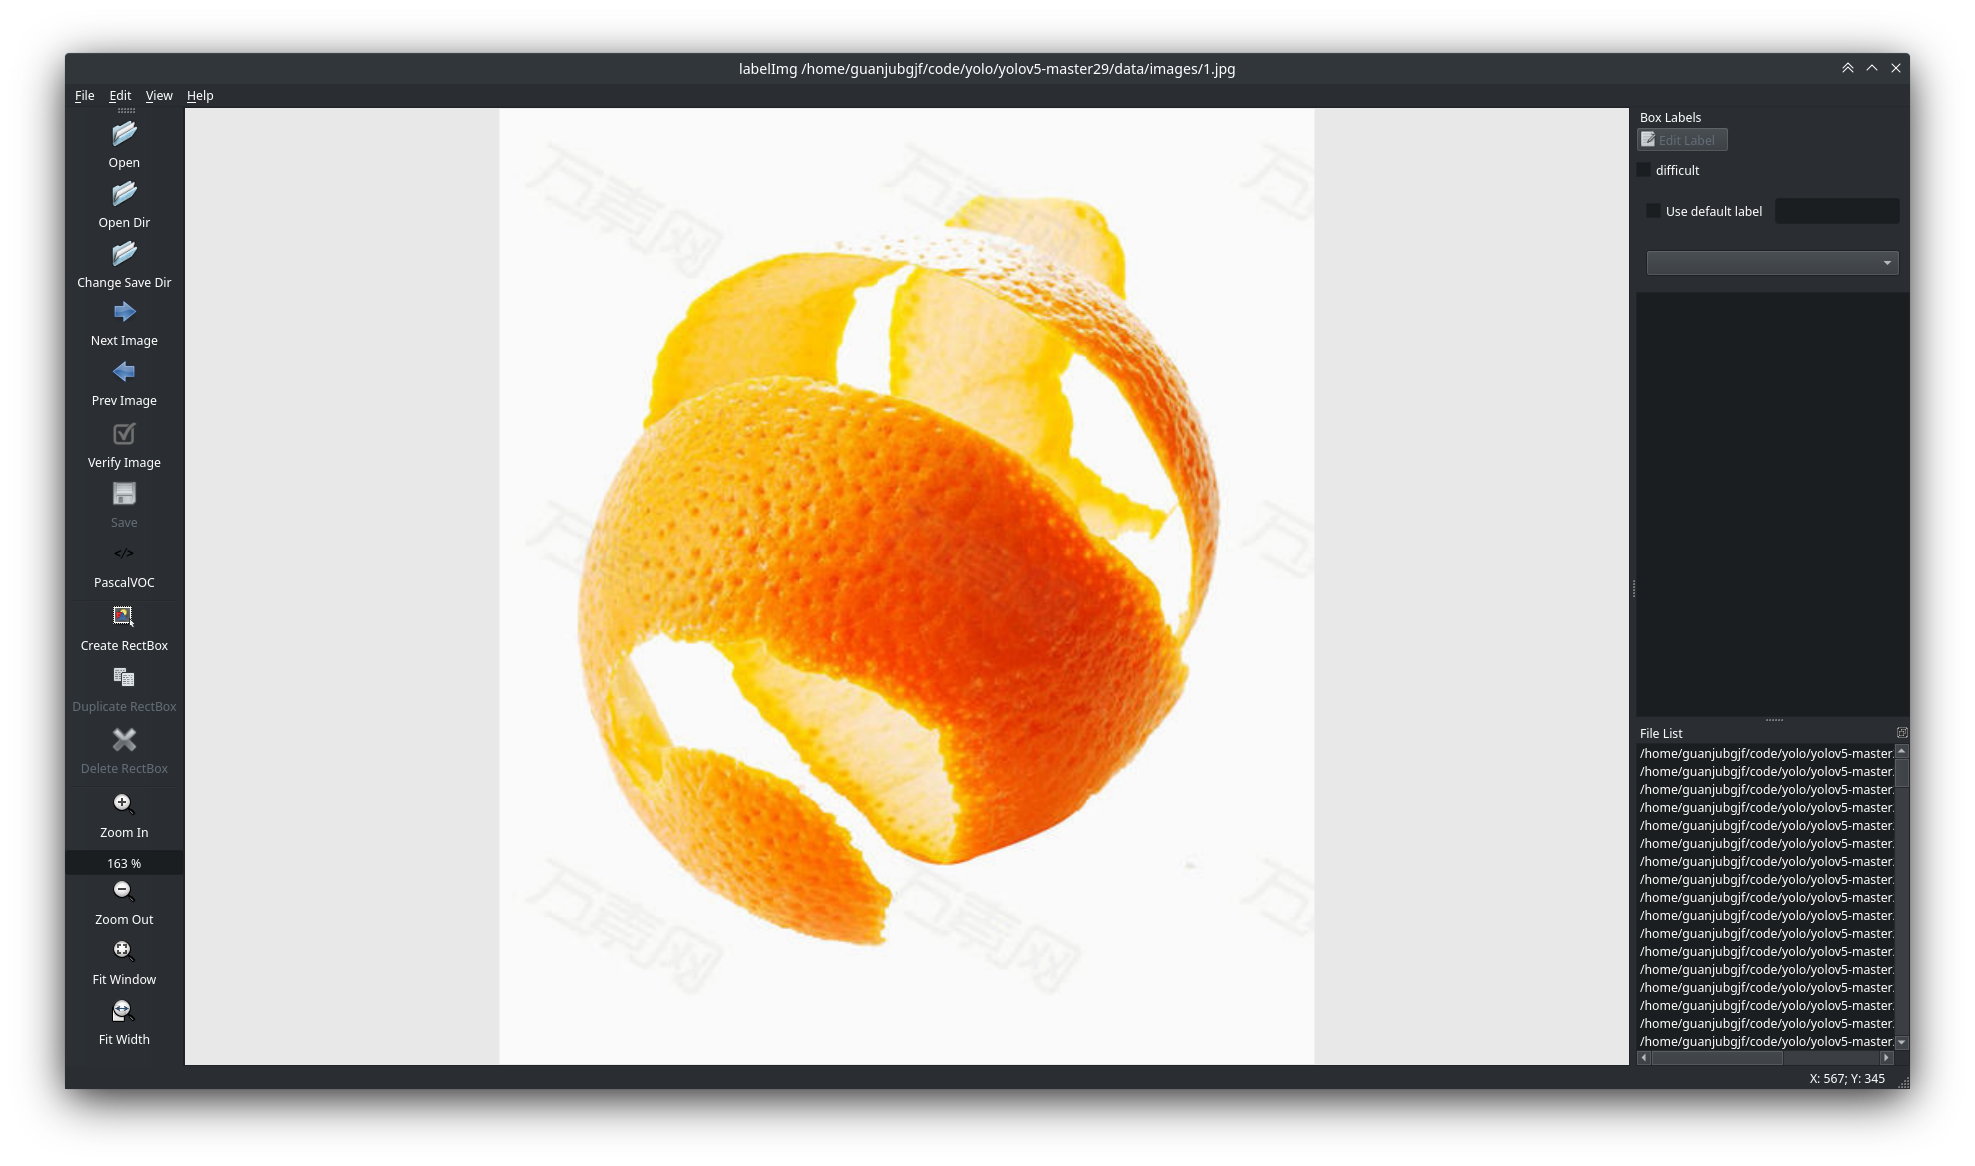
\includegraphics[width=0.8\textwidth]{figures/labelImg-window.png}
    \caption{用labelImg手动对图片打标签}
    \label{labelImg}
\end{figure}

用矩形框选目标,得到矩形四个顶点的坐标和目标的类别号作为训练数据。


\section{目录结构说明}

\begin{enumerate}
    \item 需要执行的python文件为./test.py
    \item 采用的模型为./yolov5s.pt
    \item 训练的所有模型存放于./runs/train/exp3/weights/
    \item 训练日志存放于./runs/train/exp3/
\end{enumerate}


\section{模型结构及方案设计}

yolov5s模型首先对图片采用Mosaic数据增强,并对图片进行自适应缩放,
通常缩放到$608\times 608$

\begin{figure}[H]
    \centering
    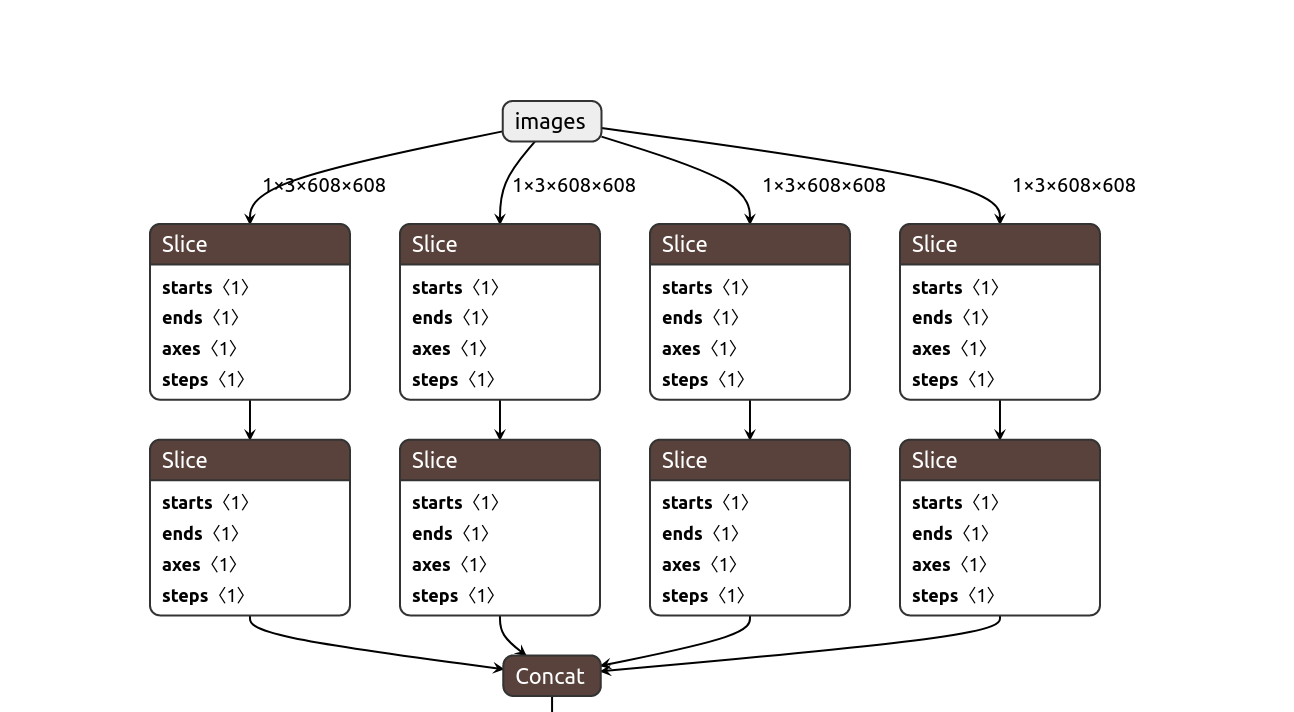
\includegraphics[width=0.8\textwidth]{figures/yolov5-structure-1.png}
\end{figure}

随后图片通过切片操作,原始608*608*3的图像变成304*304*12的特征图,
再经过一次32个卷积核的卷积操作,最终变成304*304*32的特征图。

\begin{figure}[H]
    \centering
    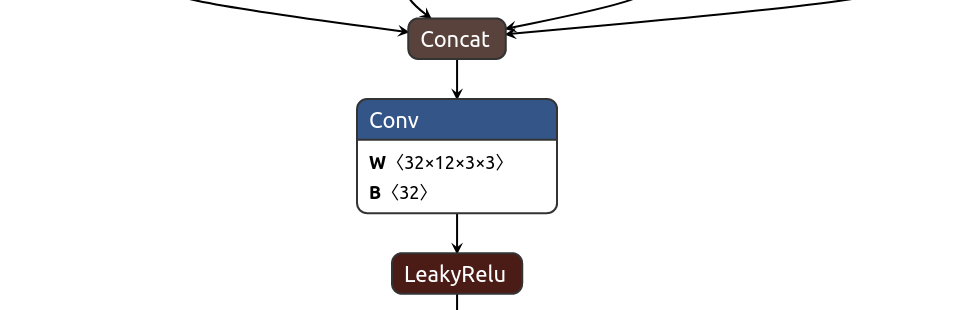
\includegraphics[width=0.8\textwidth]{figures/yolov5-structure-2.png}
\end{figure}

接下来通过模型中的第一个BottlenneckCSP结构:分为两部分,Bottlenneck以及CSP。
其中Bottleneck是一个残差结构: 先是1x1的卷积层,然后再是3x3的卷积层,
最后通过残差结构与初始输入相加。

\begin{figure}[H]
    \centering
    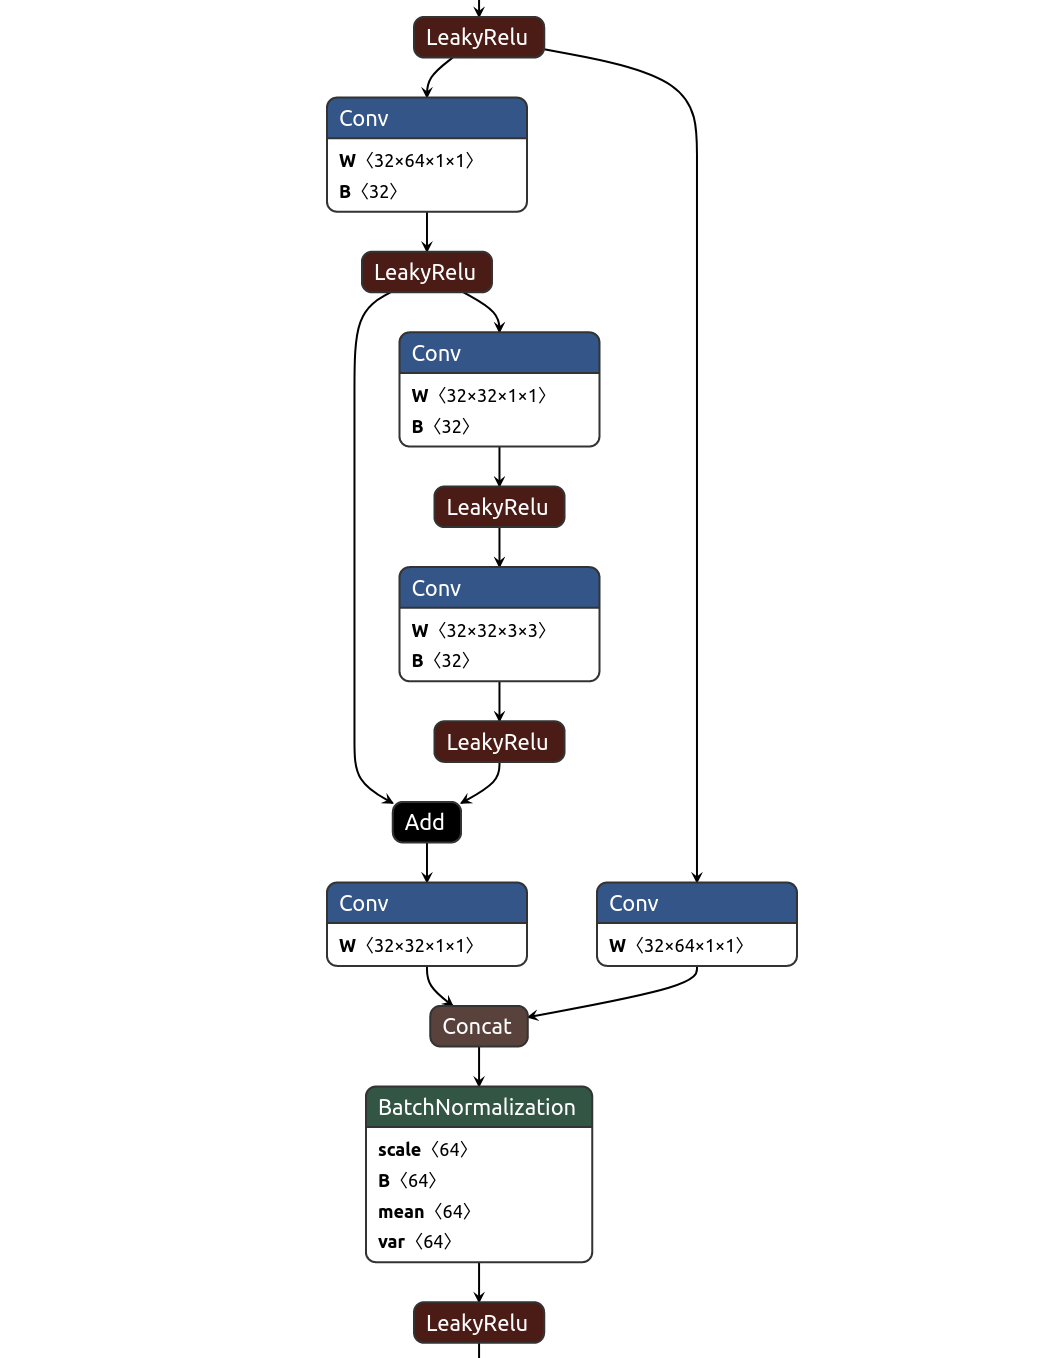
\includegraphics[width=0.8\textwidth]{figures/yolov5-structure-3.png}
\end{figure}

随后进入SPP模块,采用padding操作,移动的步长为1,从而保持图片在卷积池化操作前后尺寸不变。

\begin{figure}[H]
    \centering
    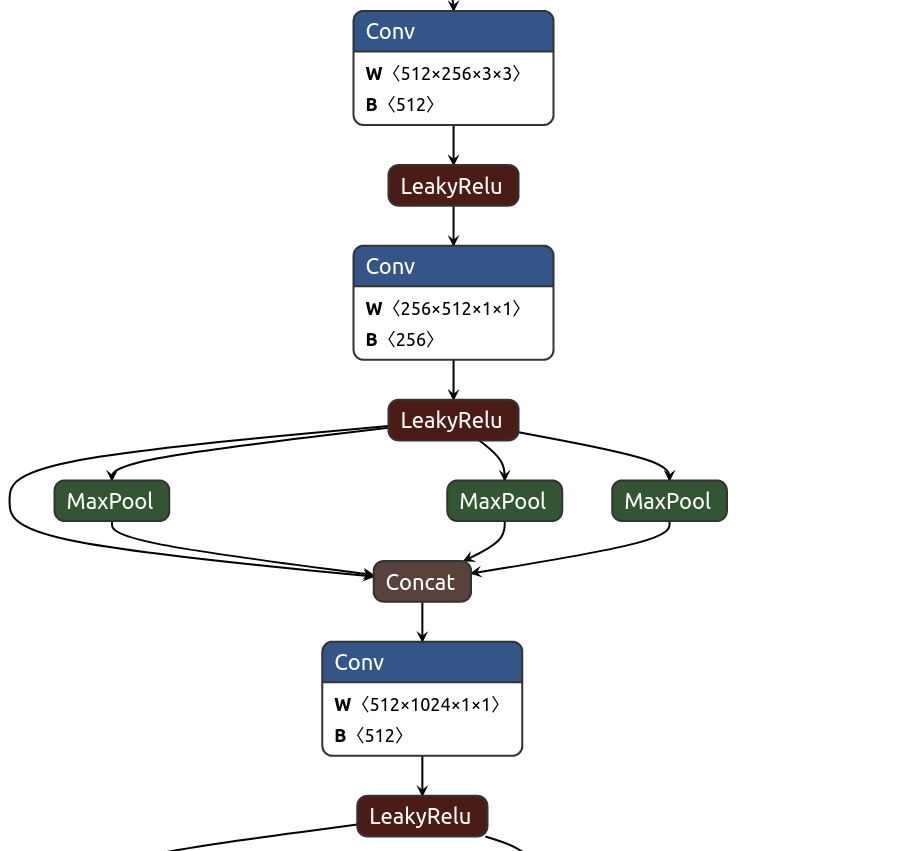
\includegraphics[width=0.8\textwidth]{figures/yolov5-structure-4.png}
\end{figure}

以上部分是yolov5s的模型主干部分,在本次实验中在一些位置进行了特征数裁剪,
其余部分均未修改。

yolov5s中采用其中的CIOU loss做Bounding box的损失函数。
CIOU考虑检测框和目标框重叠面积,并解决边界框不重合时的问题、考虑边界框中心点距离的信息,
以及边界框宽高比的尺度信息。由于CIOU效果通常较好,因此在本次实验中没有修改这个函数。

在本次实验中创建的yoloDetector类为封装了yolov5和open-cv后的目标识别功能。
在detect方法中返回检测到的目标的中心坐标和类别。


\section{训练过程}

训练时,基于预训练的轻量级yolov5s模型进行进一步的训练。

训练过程中,各个类别在测试集上的准确率、召回率如图\ref{PandR}。

\begin{figure}[H]
    \begin{minipage}[H]{0.5\linewidth}
        \centering
        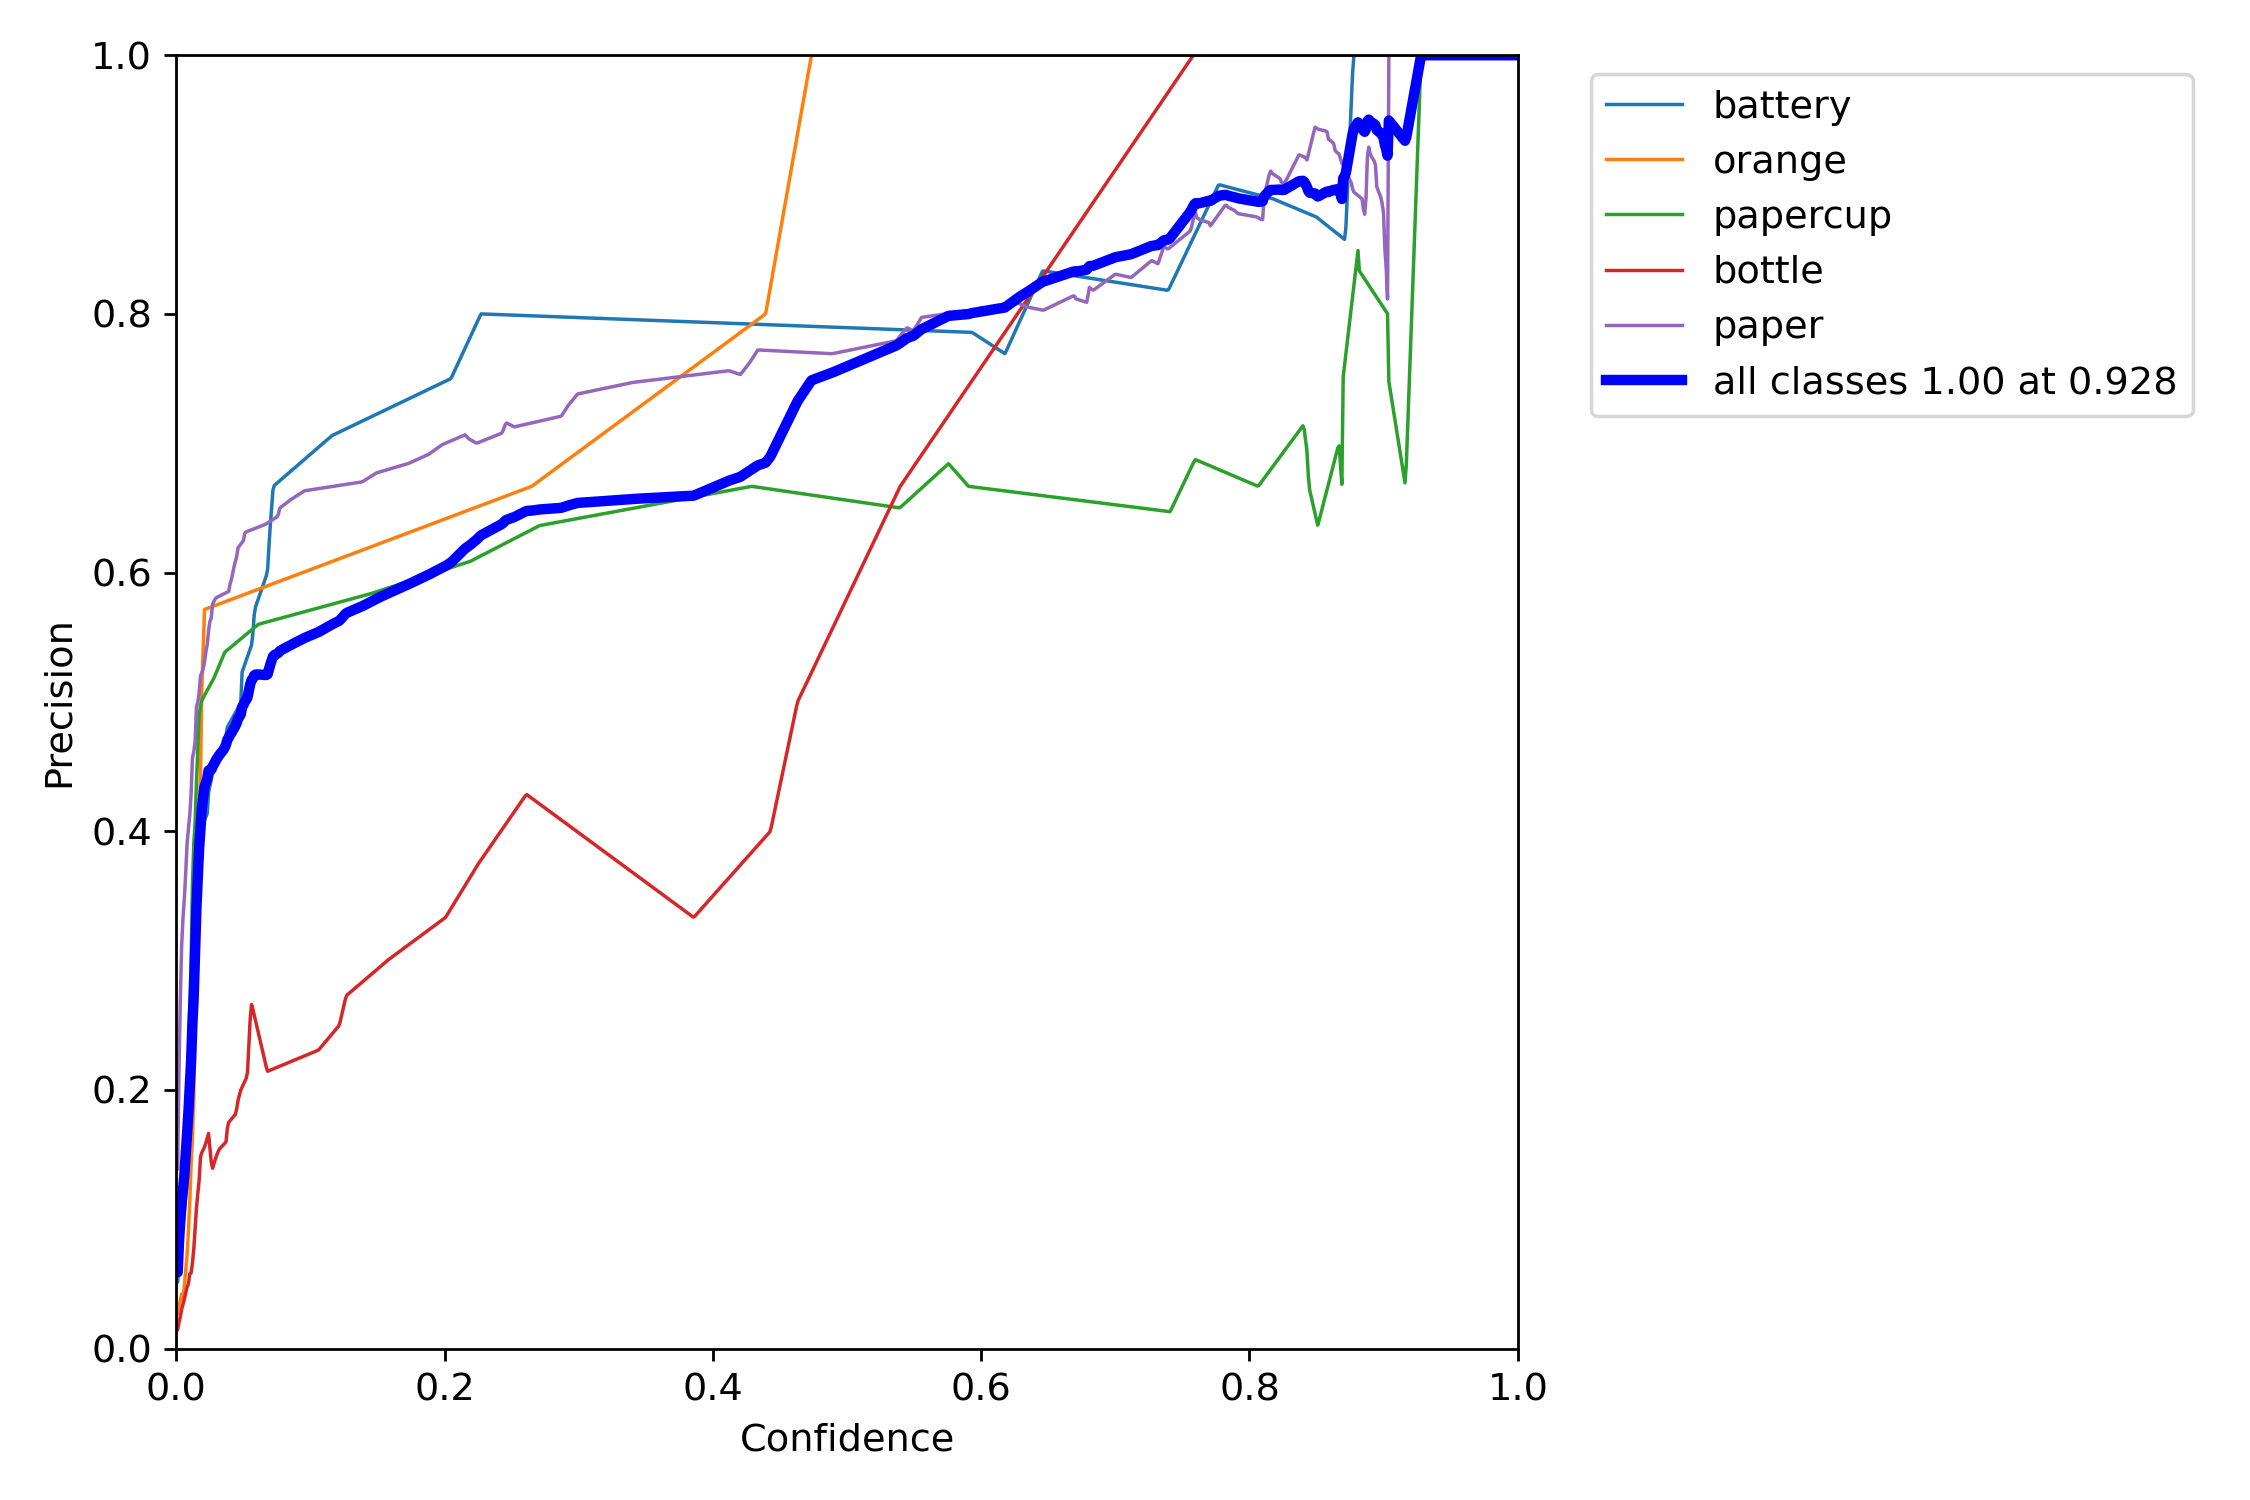
\includegraphics[width=\textwidth]{figures/P_curve.png}
        \caption{准确率}
    \end{minipage}
    \begin{minipage}[H]{0.5\linewidth}
        \centering
        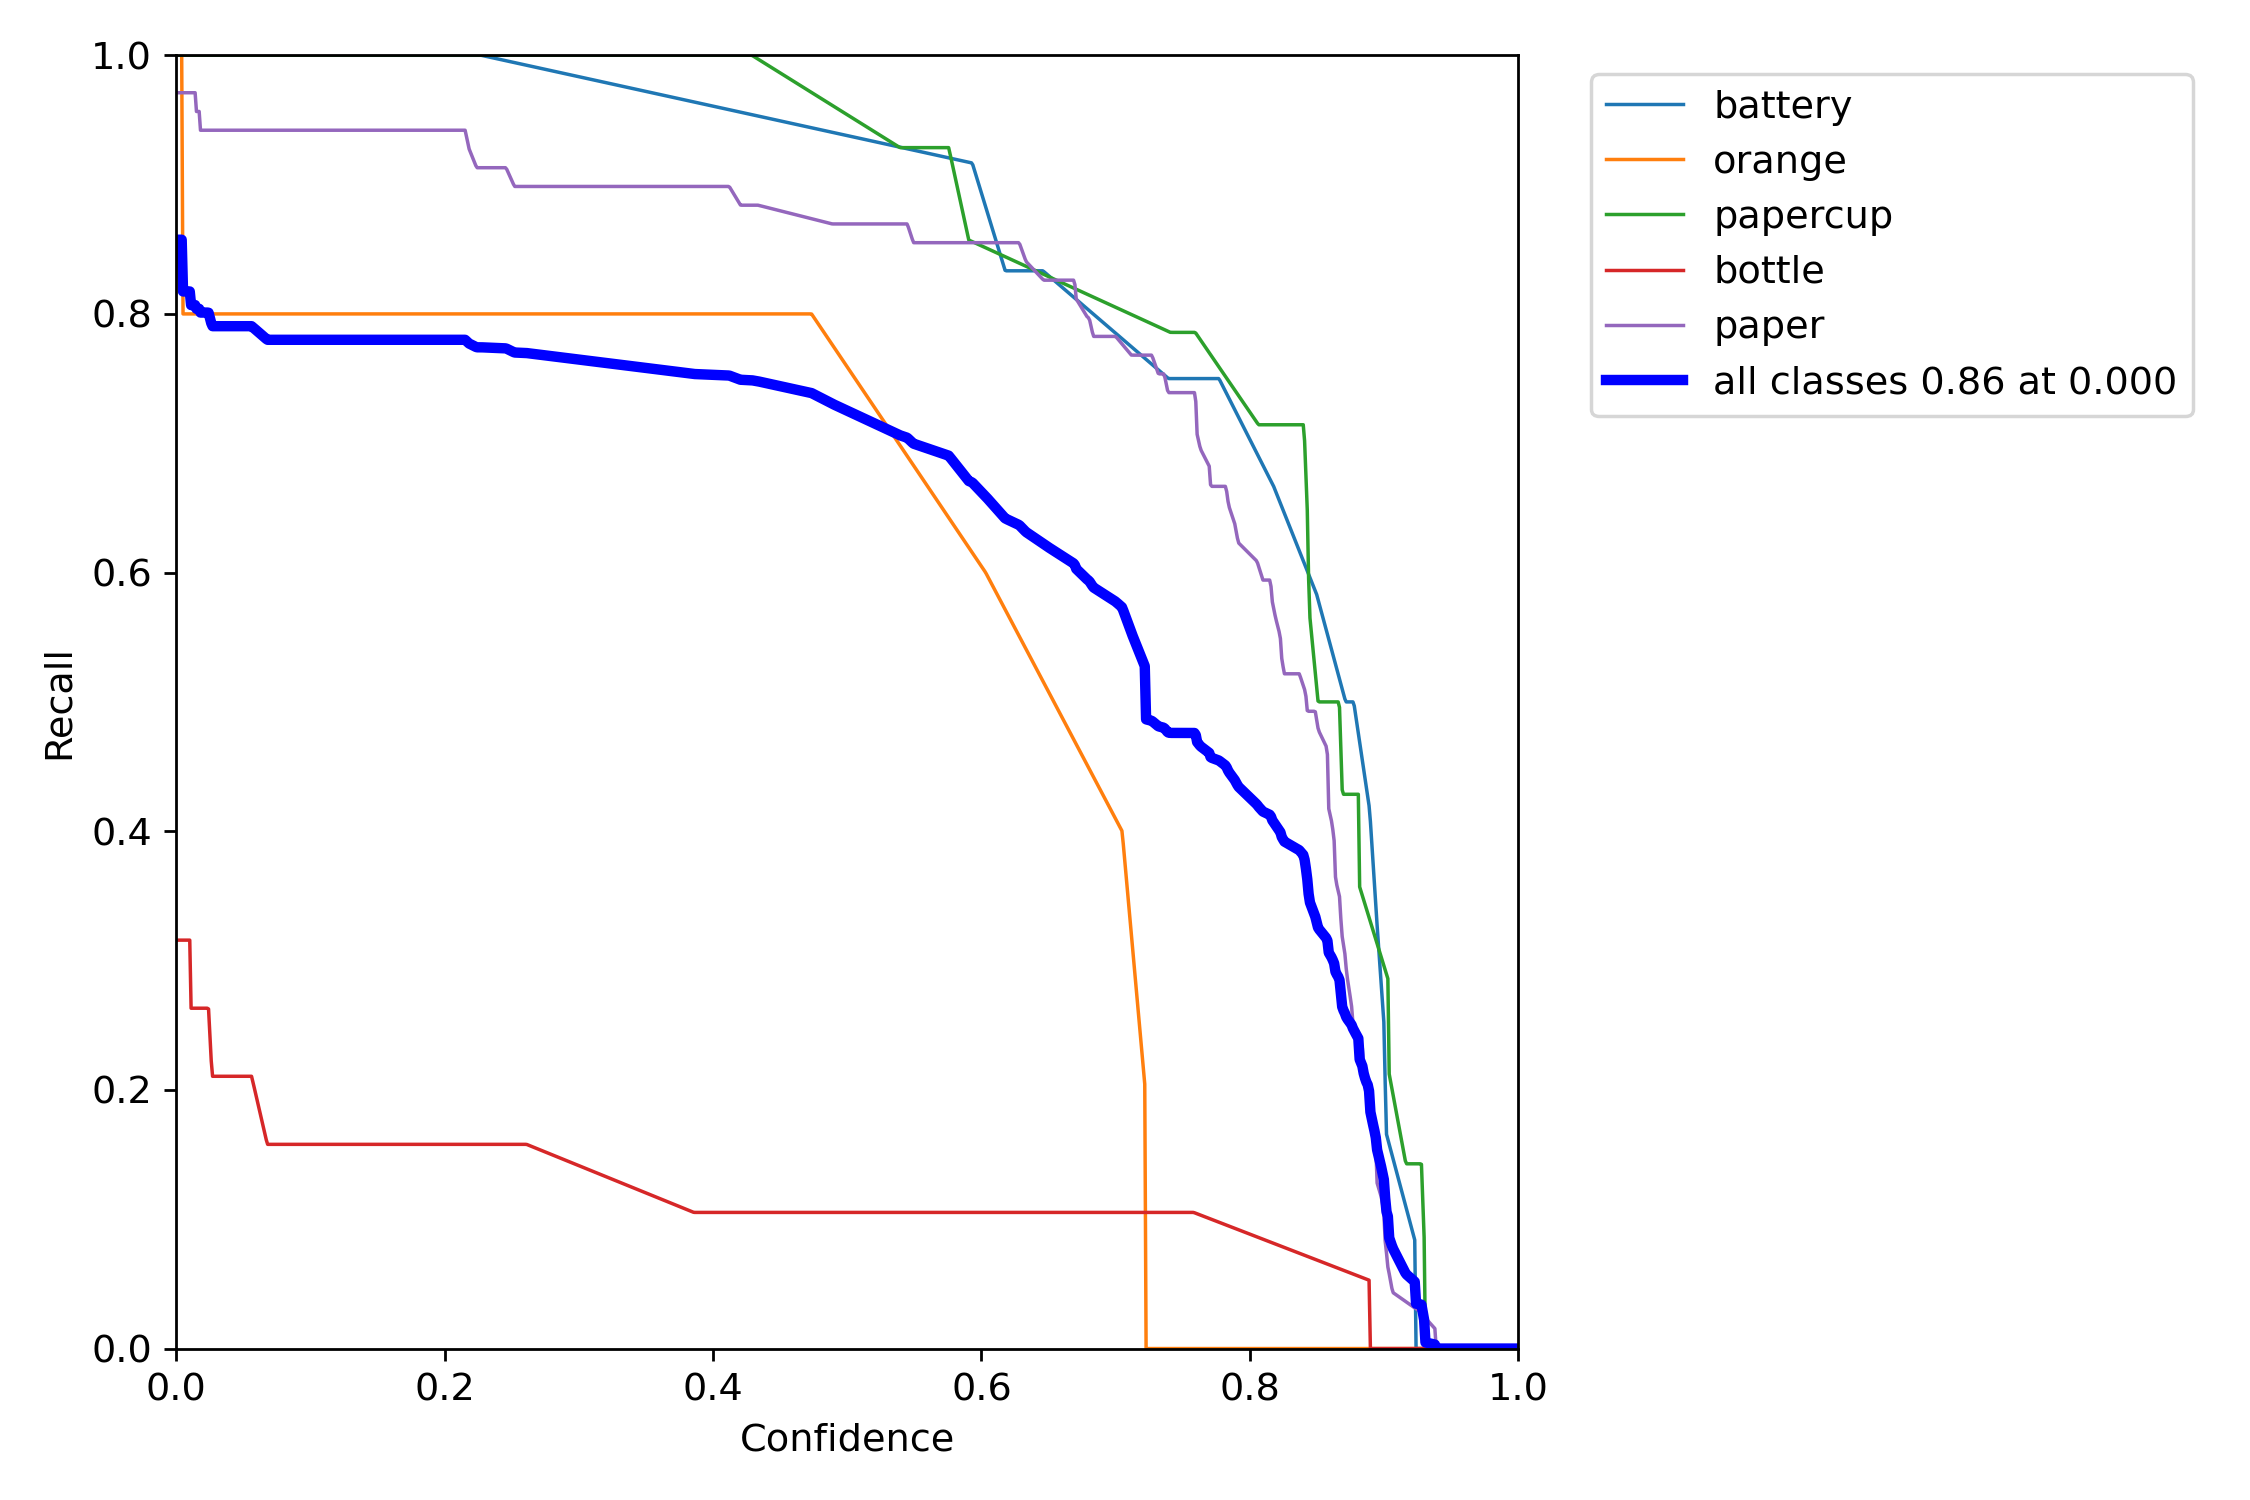
\includegraphics[width=\textwidth]{figures/R_curve.png}
        \caption{召回率}
    \end{minipage}
    \label{PandR}
    \caption{各个类别在测试集上的准确率、召回率}
\end{figure}

各个类别在测试集上的F1值和P-R曲线如图\ref{f1andPR}。

\begin{figure}[H]
    \begin{minipage}[H]{0.5\linewidth}
        \centering
        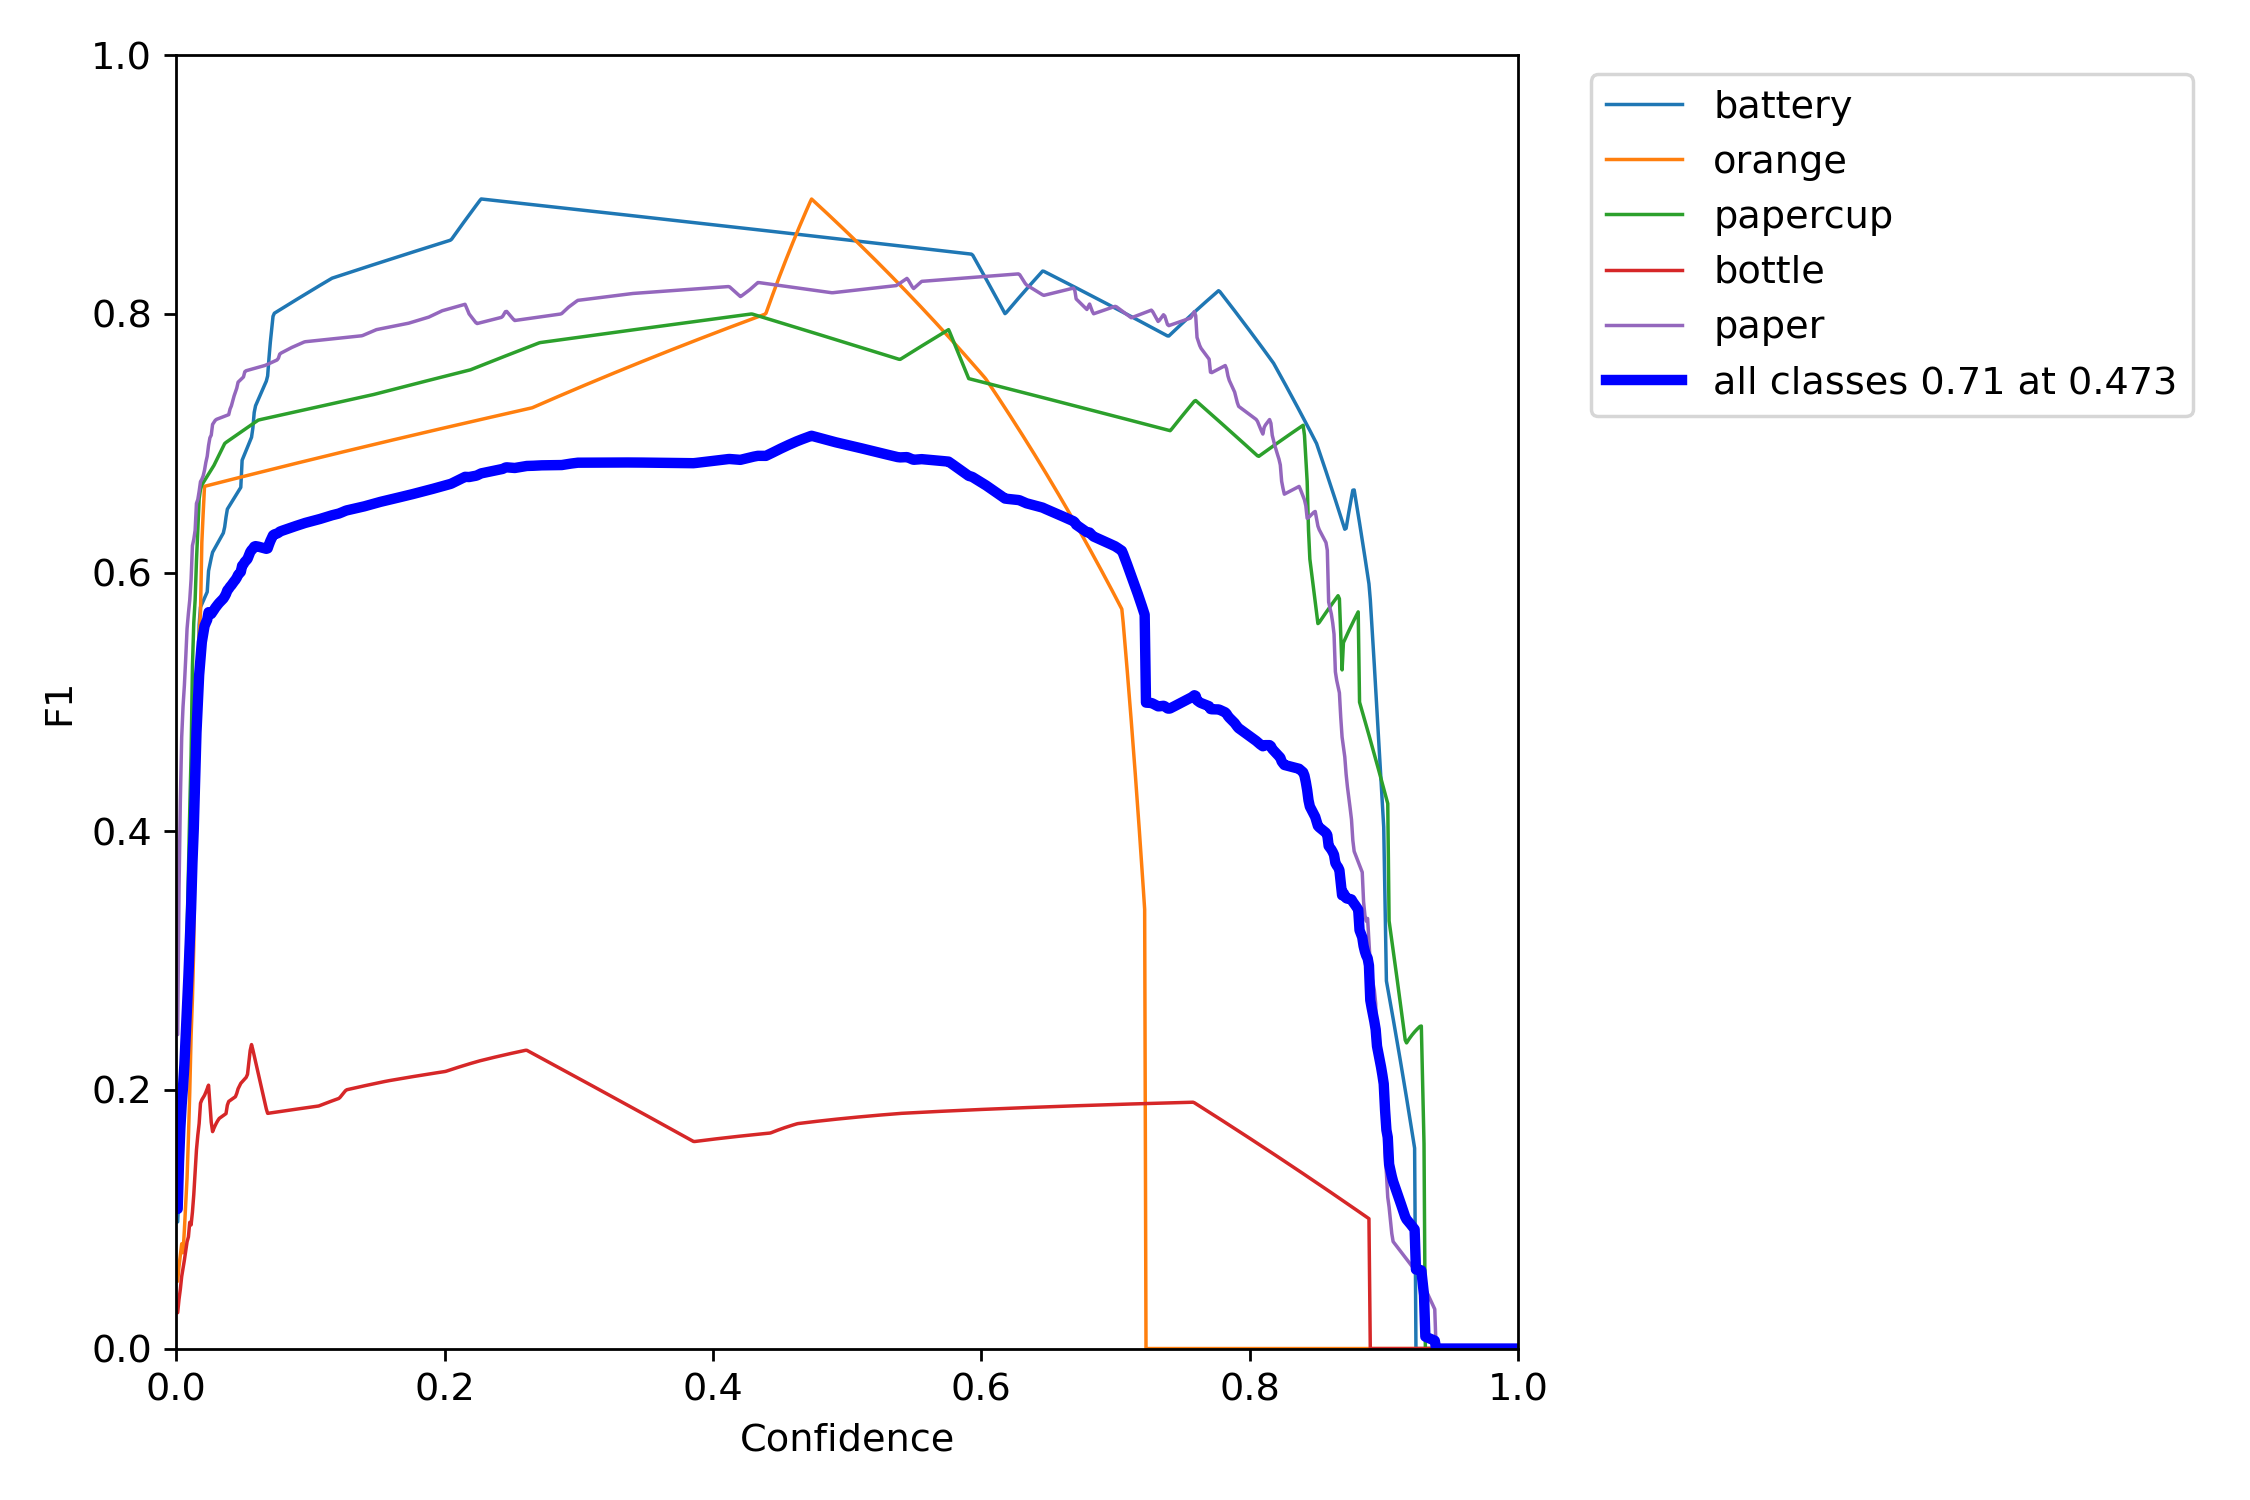
\includegraphics[width=\textwidth]{figures/F1_curve.png}
        \caption{F1值}
    \end{minipage}
    \begin{minipage}[H]{0.5\linewidth}
        \centering
        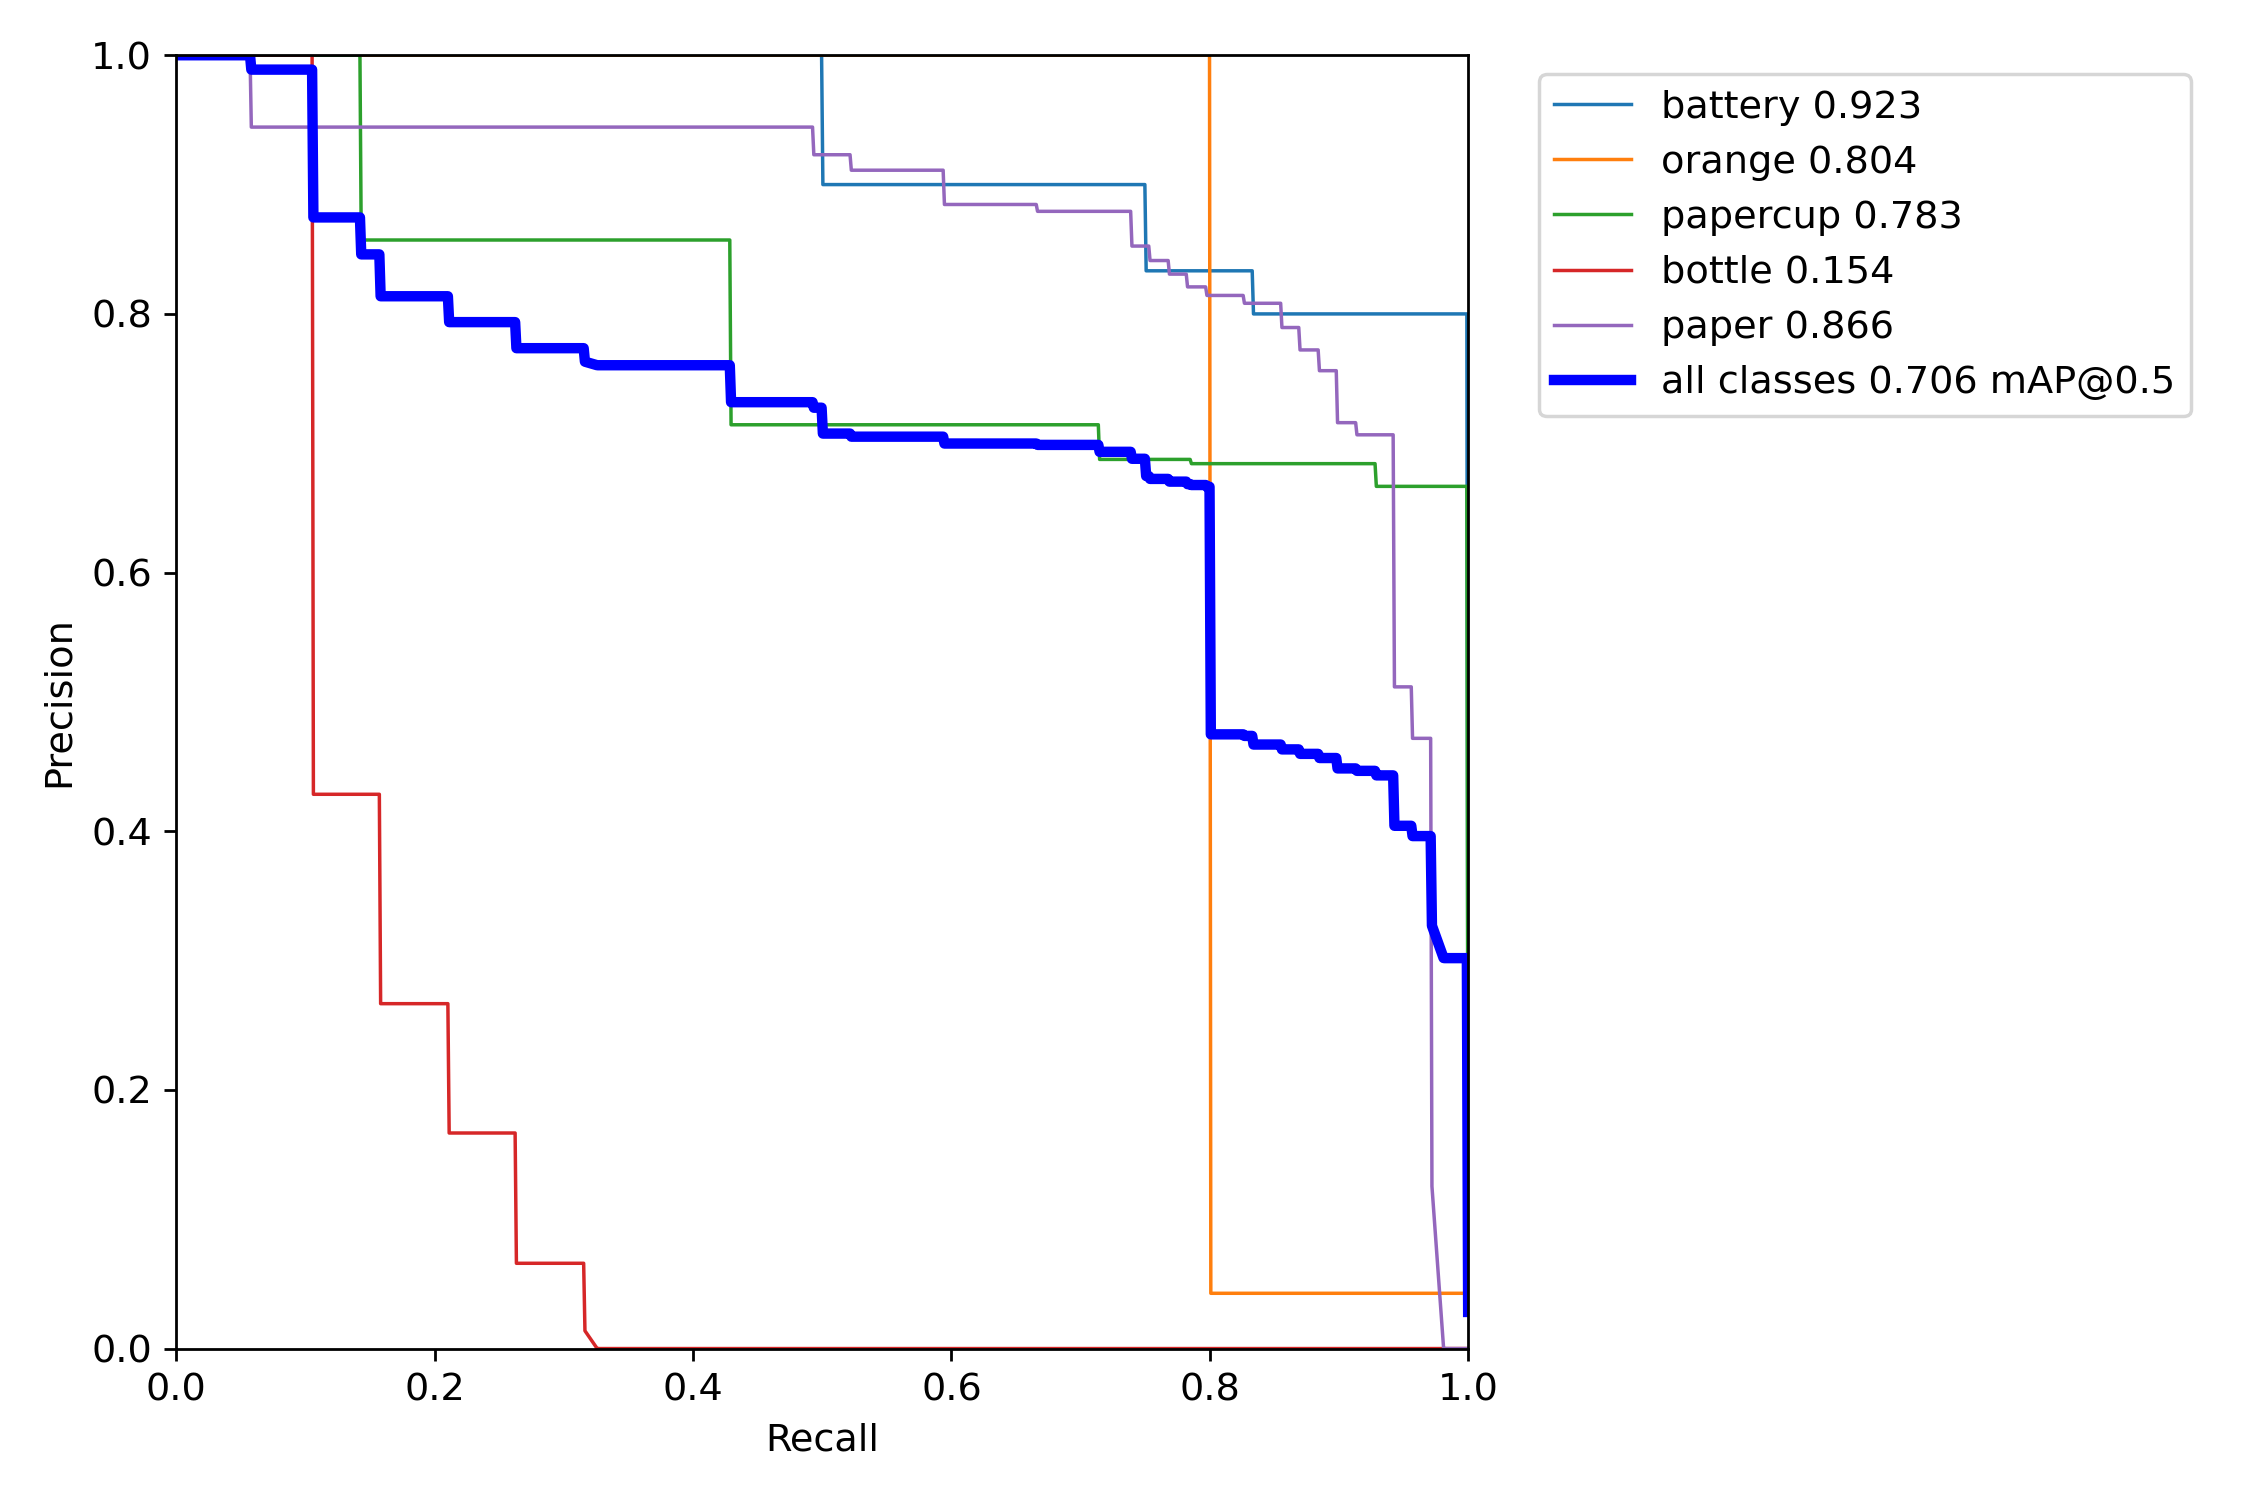
\includegraphics[width=\textwidth]{figures/PR_curve.png}
        \caption{P-R曲线}
    \end{minipage}
    \label{f1andPR}
    \caption{各个类别在测试集上的F1值和P-R曲线}
\end{figure}

总的准确率、召回率如图\ref{PandR-sum}。

\begin{figure}[H]
    \begin{minipage}[H]{0.5\linewidth}
        \centering
        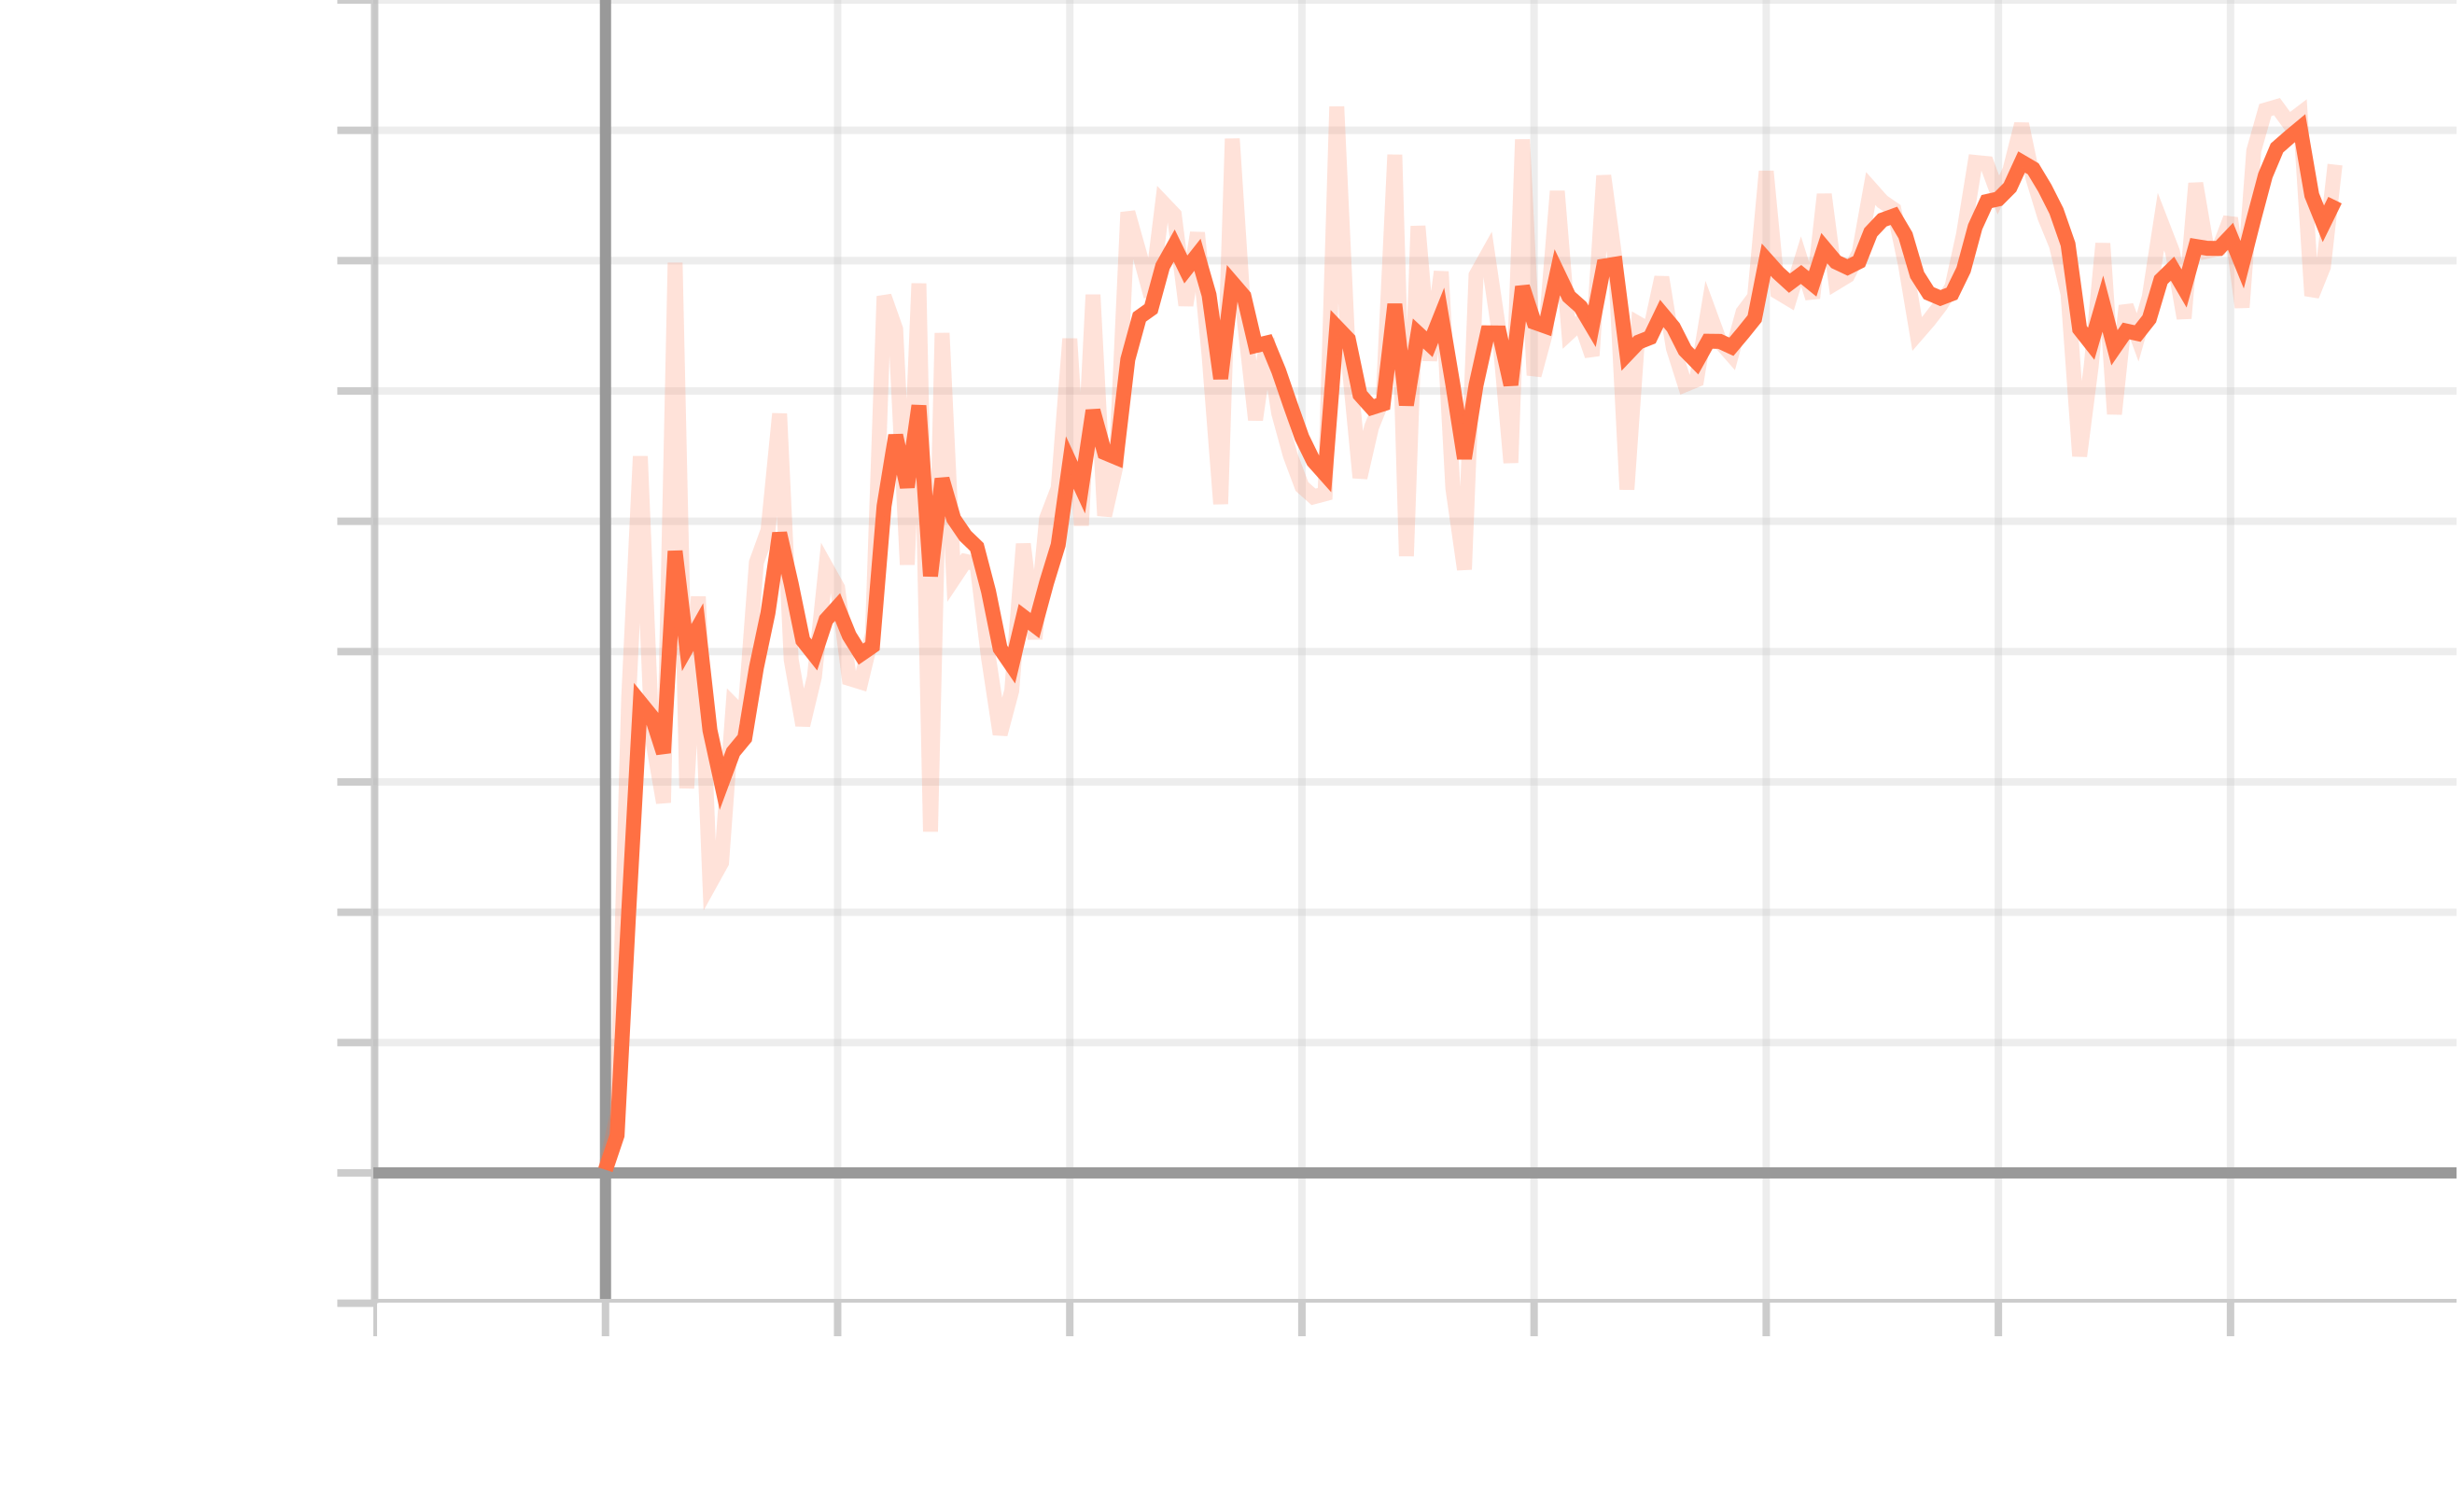
\includegraphics[width=\textwidth]{figures/metrics_precision.png}
        \caption{准确率}
    \end{minipage}
    \begin{minipage}[H]{0.5\linewidth}
        \centering
        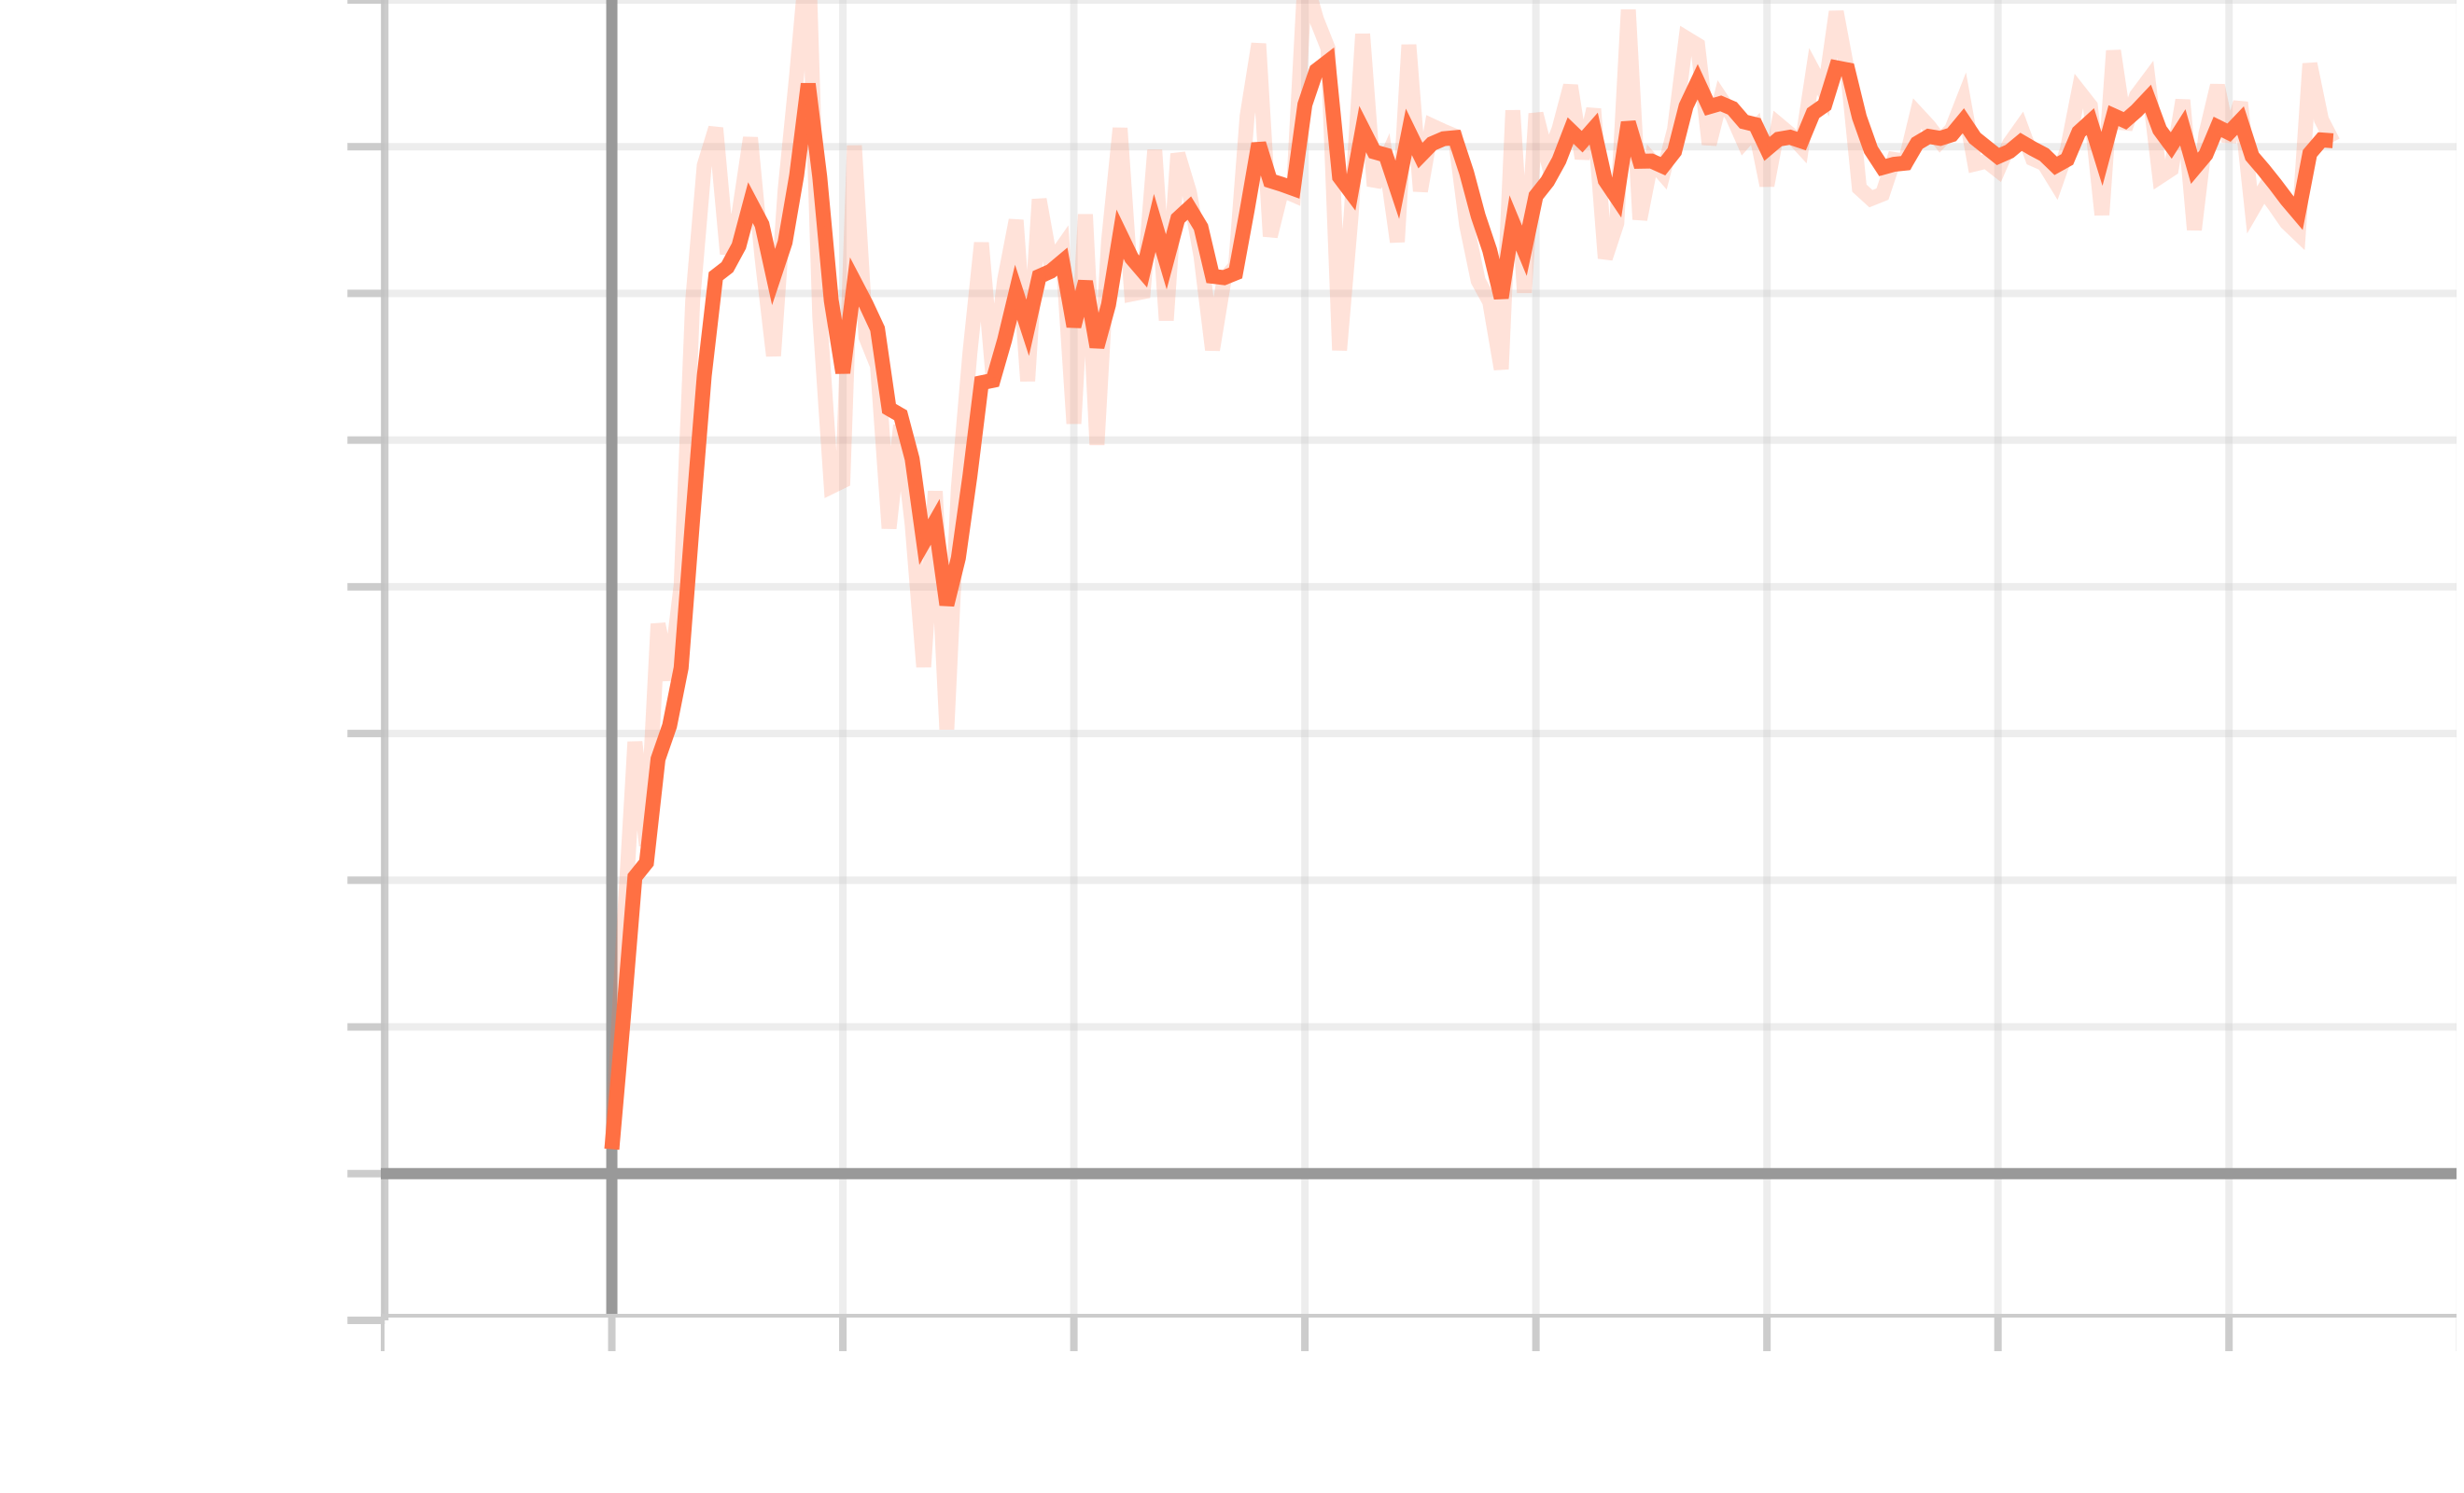
\includegraphics[width=\textwidth]{figures/metrics_recall.png}
        \caption{召回率}
    \end{minipage}
    \label{PandR-sum}
    \caption{总的准确率、召回率}
\end{figure}

在本次实验中,新学习到了mAP的概念。
在多标签图像分类任务中,图片的标签不止一个,
因此评价不能用普通单标签图像分类的标准即mean accuracy,
因此采用的是平均化的mean accuracy,即mean Average Precision,
其计算方法比较繁琐。

最终得到的所有类别上的的mAP如图\ref{mAP}。

\begin{figure}[H]
    \begin{minipage}[H]{0.5\linewidth}
        \centering
        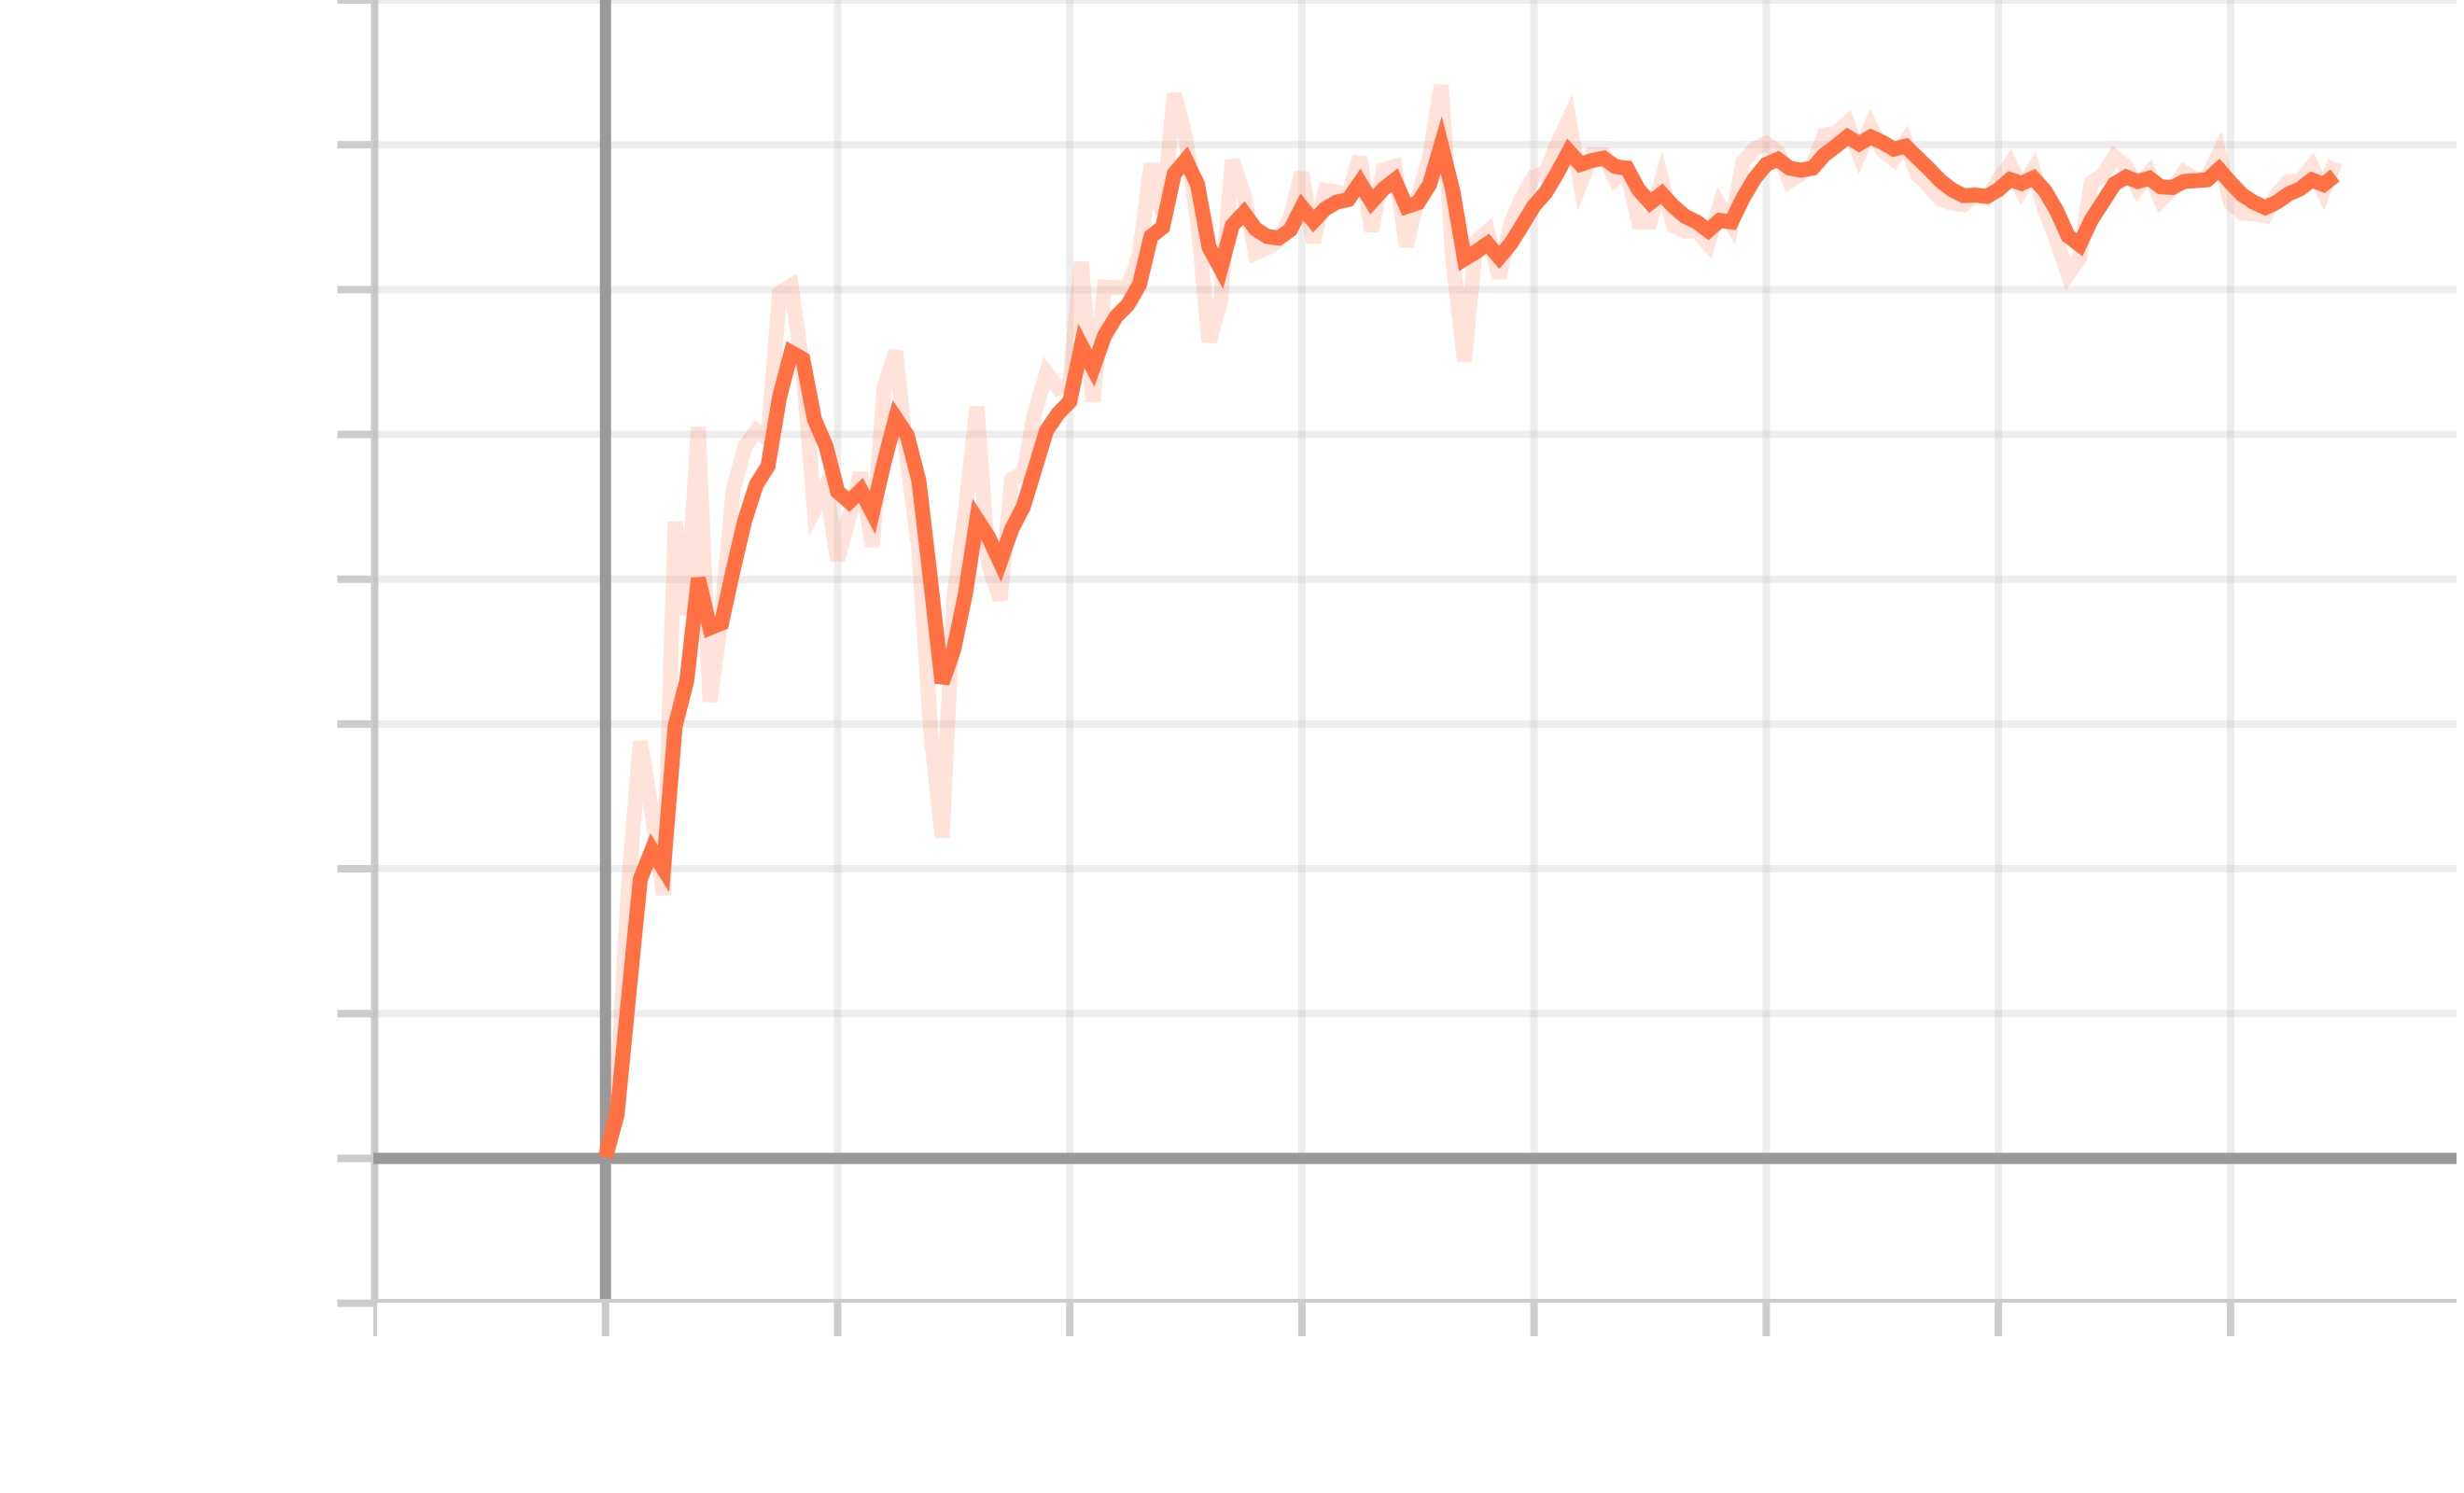
\includegraphics[width=\textwidth]{figures/metrics_mAP_0.5.png}
        \caption{mAP 0.5}
    \end{minipage}
    \begin{minipage}[H]{0.5\linewidth}
        \centering
        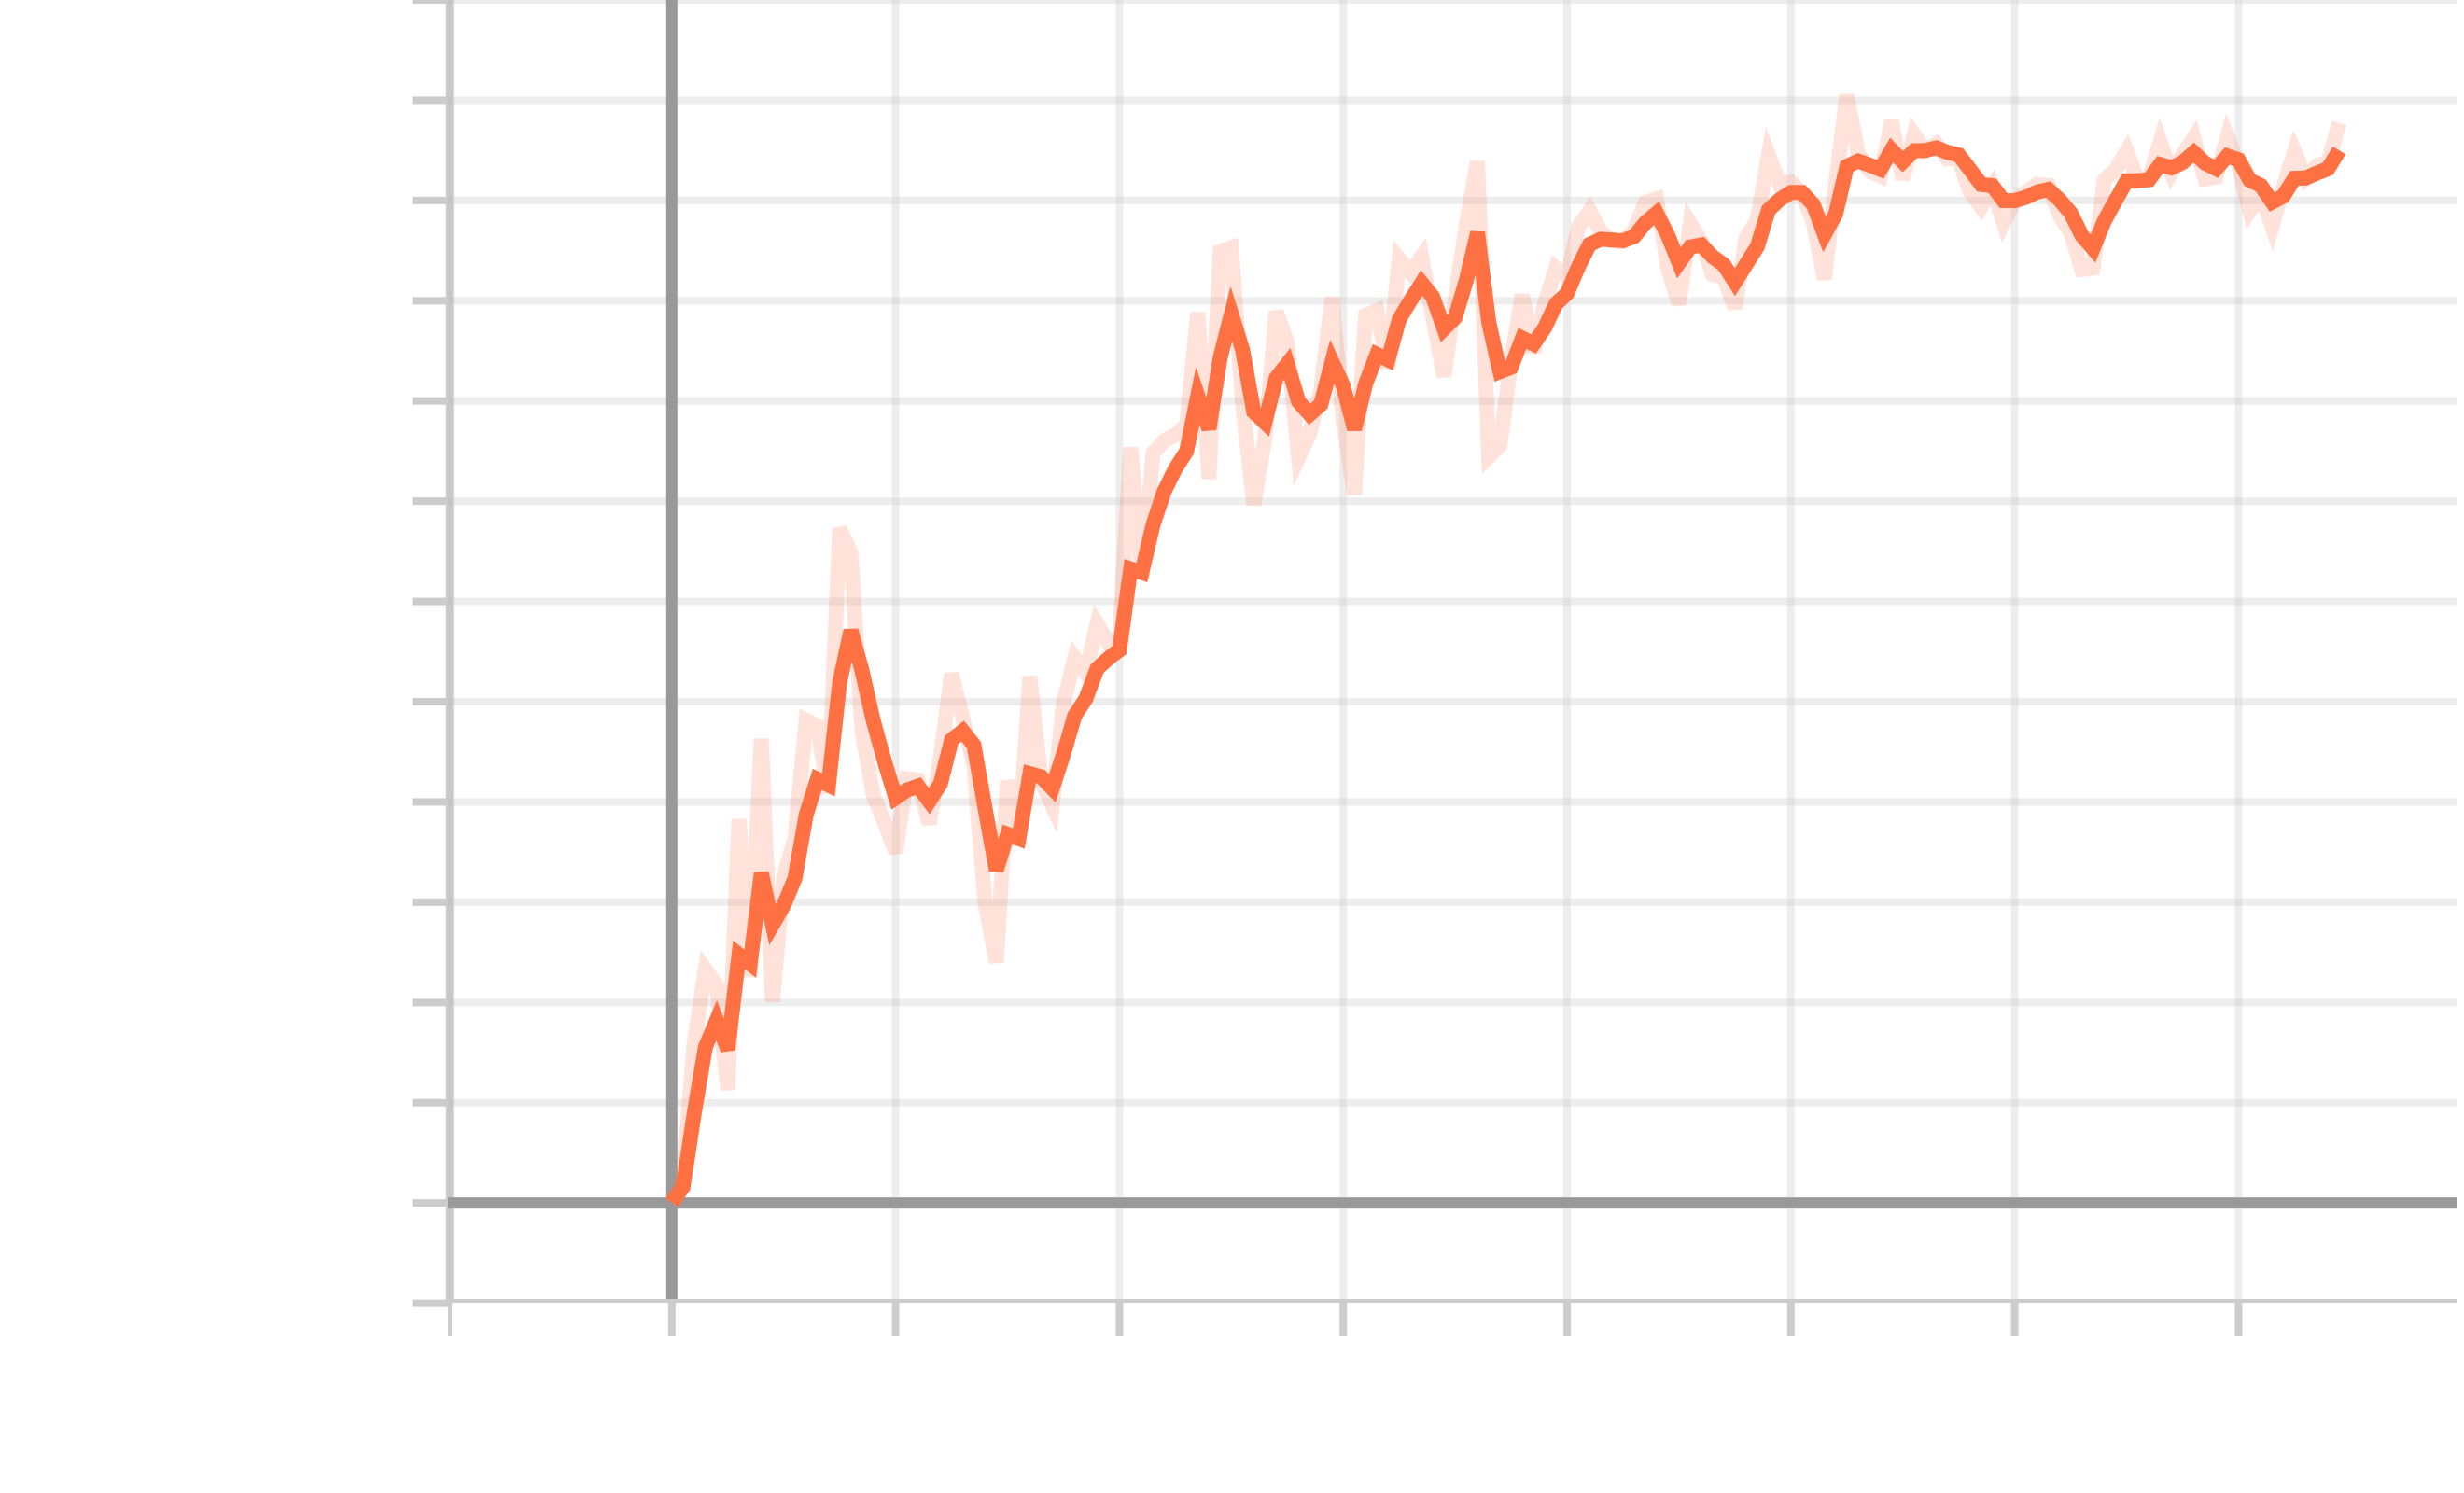
\includegraphics[width=\textwidth]{figures/metrics_mAP_0.5 0.95.png}
        \caption{mAP 0.5 0.95}
    \end{minipage}
    \label{mAP}
    \caption{所有类别上的的mAP}
\end{figure}

混淆矩阵如图\ref{confusion_matrix}

\begin{figure}[H]
    \centering
    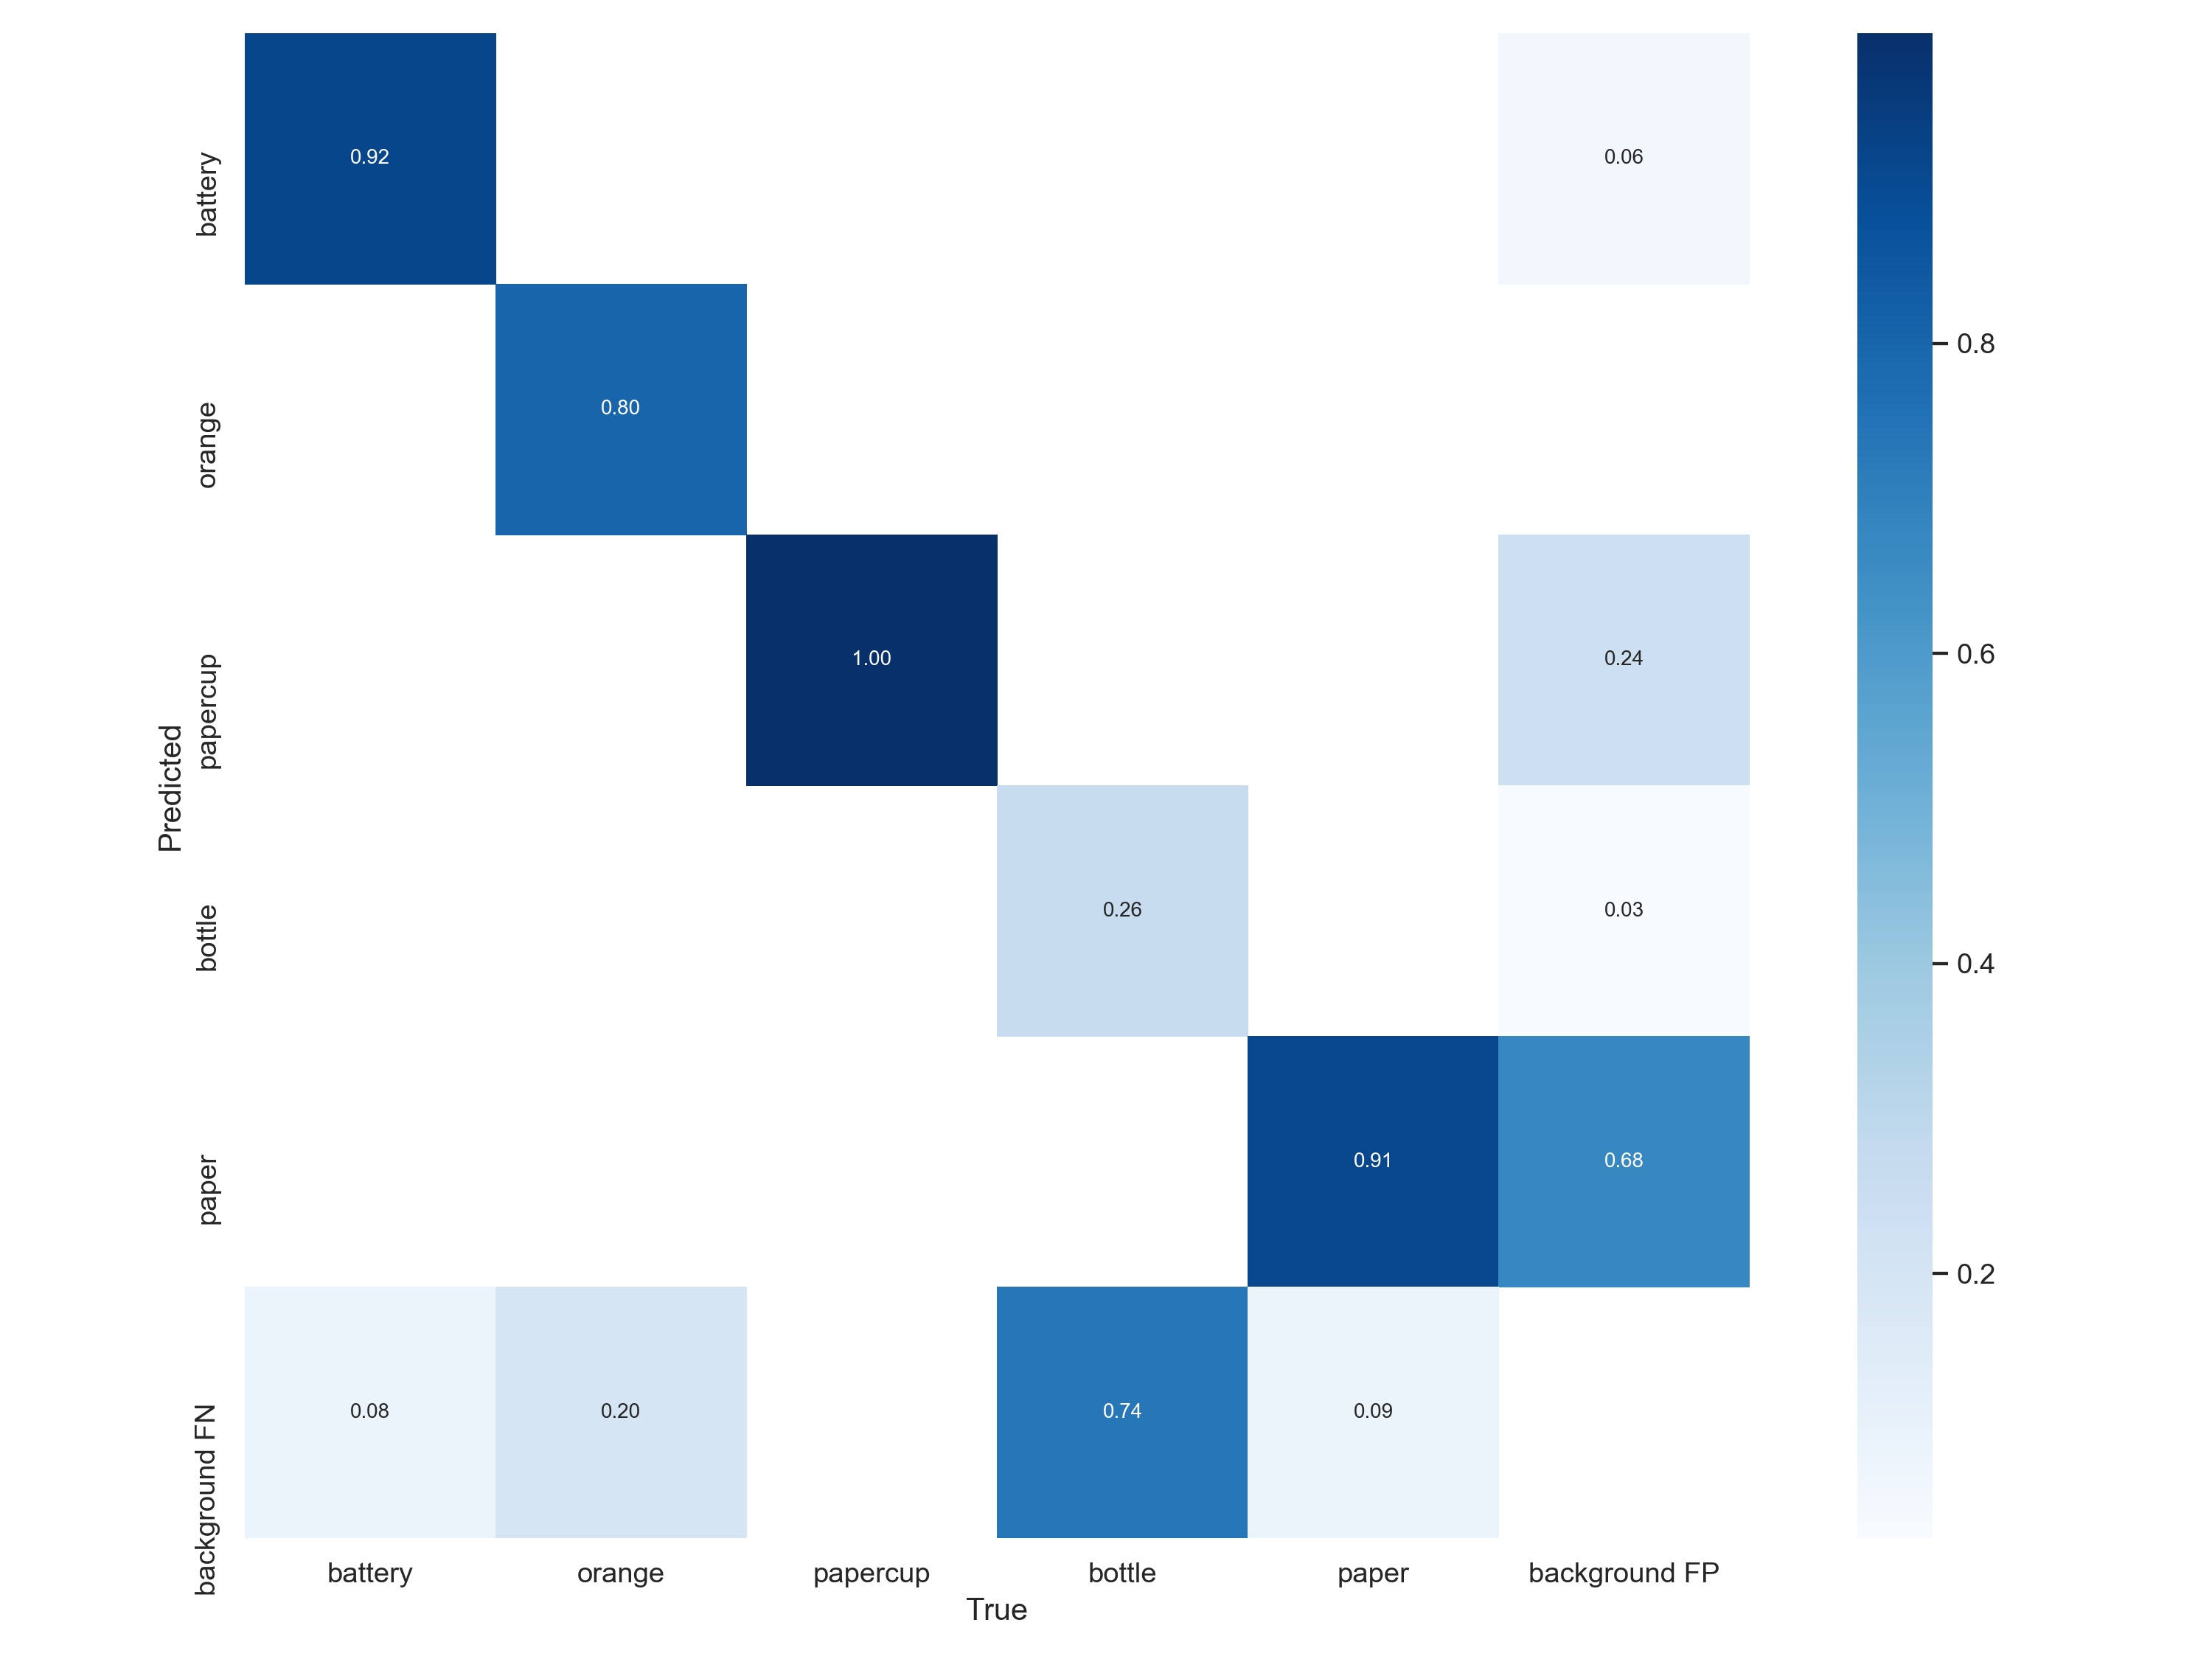
\includegraphics[width=0.8\textwidth]{figures/confusion_matrix.png}
    \caption{混淆矩阵}
    \label{confusion_matrix}
\end{figure}

由于手动打标签太慢,因此训练用的数据比较少,且数据选取可能存在分布不均等问题,
因此可能会出现一定的过拟合现象。这一点在混淆矩阵中体现较为明显。


\section{实验结果}

测试集上的识别结果如图\ref{dect}

\begin{figure}[H]
    \centering
    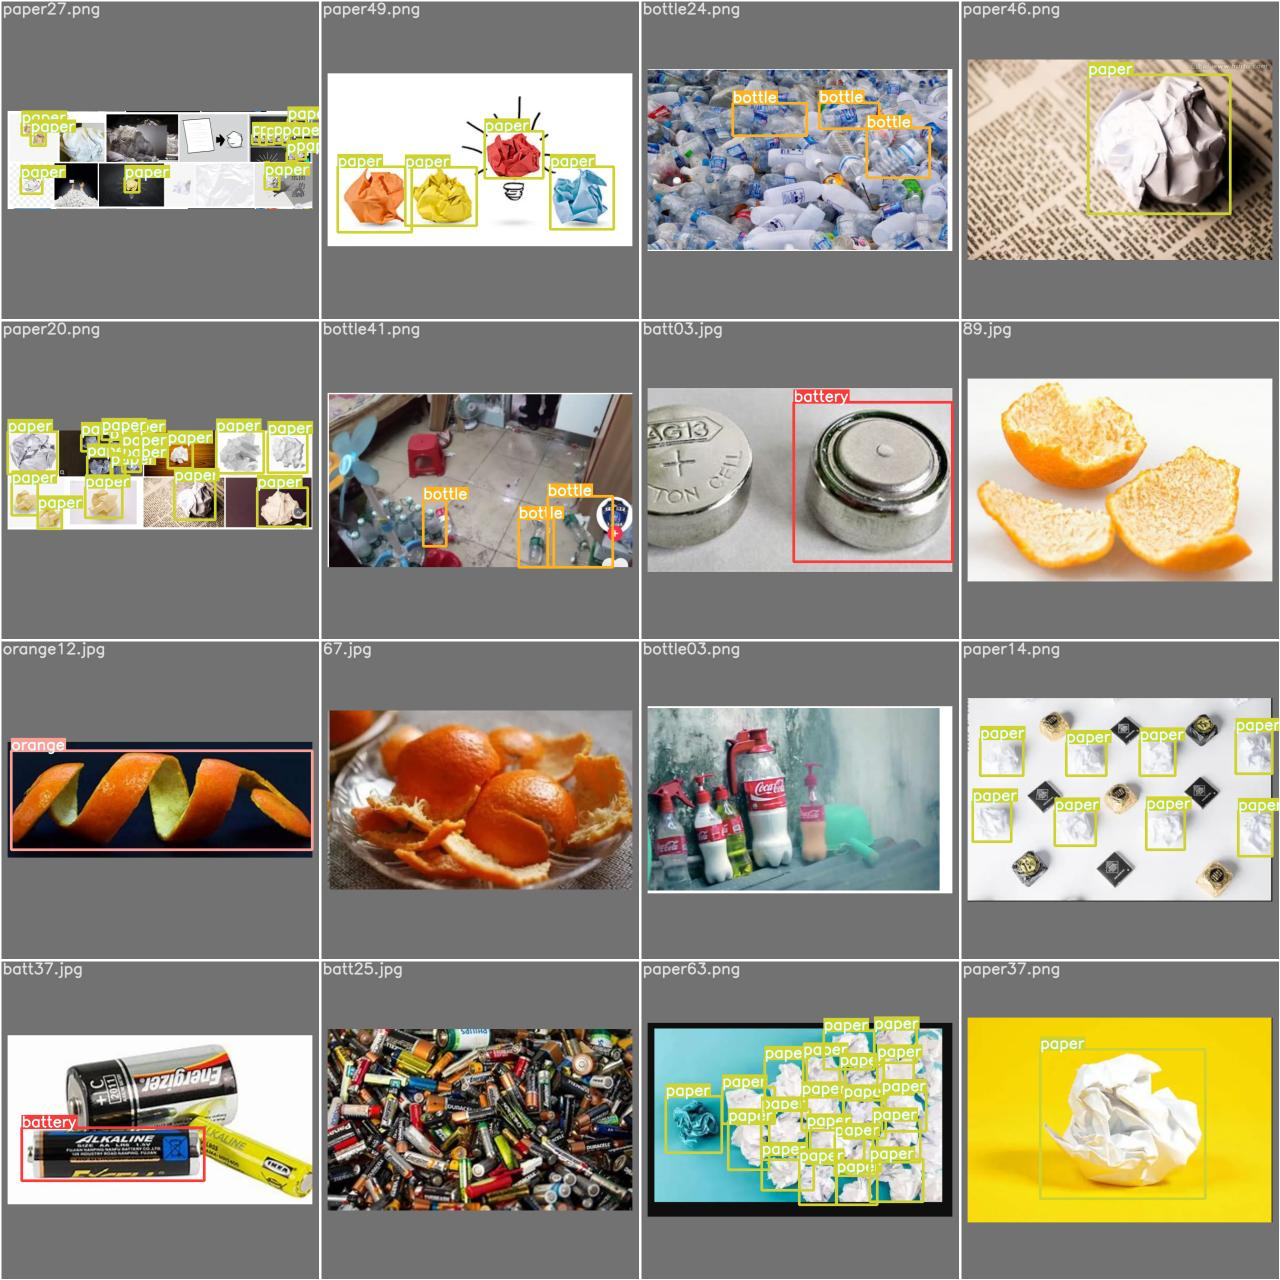
\includegraphics[width=0.8\textwidth]{figures/test_batch0_labels.jpg}
    \caption{目标识别结果}
    \label{dect}
\end{figure}

经过测试,裁剪后的框架在实际的开发板上也具有相对较高的性能和较快的速度。


\end{document}
